\documentclass[11pt,twoside]{article}
\usepackage{chadstyle}  % Loads my formatting 
\usepackage{aas_macros} % macro pour Bibtex
\usepackage{longtable,booktabs}
\usepackage{stmaryrd}
%%%%%%%%\usepackage{mdframed}
\usepackage{titlesec}
%\usepackage{hyperref}
%\usepackage[colorlinks,allcolors=blue]{hyperref}
%%%%%%%%%\usepackage{amsthm}
\usepackage{bbm}
\usepackage{ftnxtra}
\usepackage{fnpos}
\usepackage{multirow}
\usepackage{fontawesome}
\usepackage{ulem}
\usepackage{wasysym} %\permil in mathmode

\usepackage{bigints}
%%%%\usepackage[lite]{mtpro2}
\usepackage{physics}
\usepackage{scalerel}
\usepackage{mathrsfs}
\usepackage{empheq}

\usepackage{extarrows}
\usepackage{oubraces}
\usepackage{bm} % bold greak letters

%for algo
\usepackage{algorithm,algorithmic}
%\usepackage[noend]{algpseudocode}
%\algrenewcommand\algorithmicindent{0.5em}%


\usepackage{lmodern}
  \usepackage[T1]{fontenc}
  \usepackage[utf8]{inputenc}
  \usepackage{textcomp} % provides euro and other symbols
% use upquote if available, for straight quotes in verbatim environments
\IfFileExists{upquote.sty}{\usepackage{upquote}}{}
\usepackage{csquotes}

%\usepackage{tweaklist}  % I use this package as well; you may need to download

%% Shortcut commands

\usepackage[svgnames]{xcolor}%

\definecolor{maroon}{cmyk}{0, 0.87, 0.68, 0.32}
\definecolor{halfgray}{gray}{0.55}
\definecolor{ipython_frame}{RGB}{207, 207, 207}
\definecolor{ipython_bg}{RGB}{247, 247, 247}
\definecolor{ipython_red}{RGB}{186, 33, 33}
\definecolor{ipython_green}{RGB}{0, 128, 0}
\definecolor{ipython_cyan}{RGB}{64, 128, 128}
\definecolor{ipython_purple}{RGB}{170, 34, 255}


\usepackage[amsmath]{ntheorem}
\usepackage[ntheorem]{mdframed}
\newmdtheoremenv[linewidth=5pt, linecolor=Gainsboro!75!Lavender, topline=false, bottomline=false, skipabove=15pt, skipbelow=20pt]{thm}{\color{ChadBlue}Théorème}

\newmdtheoremenv[linewidth=5pt, linecolor=Gainsboro!75!Lavender, topline=false, bottomline=false, skipabove=15pt, skipbelow=20pt]{lemme}{\color{ChadBlue}Lemme}

\newmdtheoremenv[linewidth=5pt, linecolor=Gainsboro!75!Lavender, topline=false, bottomline=false, skipabove=15pt, skipbelow=20pt]{definition}{\color{ChadBlue}Définition}

\newmdtheoremenv[linewidth=5pt, linecolor=Gainsboro!75!Lavender, topline=false, bottomline=false, skipabove=15pt, skipbelow=20pt]{propriete}{\color{ChadBlue} Propriété}


%   \theoremclass{Theorem}
%\newtheorem{proposition}{\color{ChadBlue} Théorème}
%\newtheorem{lemme}{\color{ChadBlue} Lemme}
%\newtheorem{definition}{\color{ChadBlue} Définition}

\newcommand{\Proof}[2]{{\hspace{-\parindent} {\color{ChadBlue}\bf Démonstration}~\ref{#1}.}
{#2}\hfill$\blacksquare$ \\ \vspace{.1in}}

%\newcosecnumdepthmmand{\proptitle}[1]{\color{ChadBlue} \textnormal{(#1):}}
%\newtheorem{proposition}{\color{ChadGreen} Proposition}
%\newcommand{\assume}[2]{{\bf{Assumption #1}} (#2)} 
%\newcommand{\clr}[1]{{\color{ChadBlue} #1}}
%\newcommand{\clrg}[1]{{\color{ChadGreen} #1}}
%\newcommand{\Proof}[2]{\newline {\hspace{-\parindent} {\color{ChadGreen}\bf Proof of Proposition}~\ref{#1}.}
%{\color{ChadBlue} #2} \vspace{.1in}}

% If you've loaded *tweaklist.sty* above, uncomment these lines:
% Adjust spacing in itemize/enumerate; see tweaklist.sty
%\renewcommand{\enumhook}{\setlength{\topsep}{2pt}%
%  \setlength{\itemsep}{0pt}}
%\renewcommand{\itemhook}{\setlength{\topsep}{2pt}%
%  \setlength{\itemsep}{0pt}}

\ifnum 0\ifxetex 1\fi\ifluatex 1\fi=0 % if pdftex
  \usepackage[shorthands=off,main=french]{babel}
\else
    % See issue https://github.com/reutenauer/polyglossia/issues/127
  \renewcommand*\familydefault{\sfdefault}
    % load polyglossia as late as possible as it *could* call bidi if RTL lang (e.g. Hebrew or Arabic)
  \usepackage{polyglossia}
  \setmainlanguage[]{french}
\fi

\providecommand{\tightlist}{%
  \setlength{\itemsep}{0pt}\setlength{\parskip}{0pt}}

\setcounter{secnumdepth}{4}
\setcounter{tocdepth}{3}

\titleformat{\paragraph}
{\normalfont\normalsize\bfseries}{\theparagraph}{1em}{}
\titlespacing*{\paragraph}
{0pt}{0pt}{0pt}
%{0pt}{3.25ex plus 1ex minus .2ex}{1.5ex plus .2ex}

\usepackage{setspace}
\setstretch{1.2}

%eviter les lignes blanches
\raggedbottom

\newcommand*\widefbox[1]{\fbox{\hspace{2em}#1\hspace{2em}}}
%\newcommand*\widefbox[1]{{\setlength\fboxsep{10pt}\fbox{\hspace{0.5em}#1\hspace{0.5em}}}}

\newcommand{\lanczos}{\texttt{Lanczos}}
\newcommand{\sklearn}{\texttt{scikit-learn}}
\newcommand{\itemb}{\item[$\bullet$]}
\newcommand*\textitbf[1]{\textit{\textbf{#1}}}
%\def\boxcar{{\mbox{$\Pi$}}}
\DeclarePairedDelimiter\ceil{\lceil}{\rceil}
\DeclarePairedDelimiter\floor{\lfloor}{\rfloor}
\DeclarePairedDelimiterX{\Iintv}[1]{\llbracket}{\rrbracket}{\iintvargs{#1}}
\NewDocumentCommand{\iintvargs}{>{\SplitArgument{1}{,}}m}
{\iintvargsaux#1} %
\NewDocumentCommand{\iintvargsaux}{mm} {#1\mkern1.5mu..\mkern1.5mu#2}
\newcommand{\fcc}[1]{\widehat{#1}^{\raisebox{1pt}{\,\scriptsize$\ast$}}}

\newcommand{\Av}[1] {\underset {#1} {\rm Ave}\,}
%\newcommand{\sinc}{\mathrm{sinc}}
\DeclareMathOperator{\sinc}{sinc}
\DeclareMathOperator{\sincp}{sincp}
\DeclareMathOperator{\D}{D}
\DeclareMathOperator{\comb}{\raisebox{\depth}{\rotatebox{270}{$\exists$}}}
\DeclareMathOperator{\boxcar}{{\mbox{$\Pi$}}}
\DeclareMathOperator{\Si}{Si}
%\DeclareMathOperator{\si}{si}

\newcommand{\nn}{\nonumber}


\usepackage{stackengine}
%\stackMath
%\def\hatgap{2pt}
%\def\subdown{-2pt}
%\newcommand\reallywidehat[2][]{%
%\renewcommand\stackalignment{l}%
%\stackon[\hatgap]{#2}{%
%\stretchto{%
%    \scalerel*[\widthof{$#2$}]{\kern-.6pt\bigwedge\kern-.6pt}%
%    {\rule[-\textheight/2]{1ex}{\textheight}}%WIDTH-LIMITED BIG WEDGE
%}{0.5ex}% THIS SQUEEZES THE WEDGE TO 0.5ex HEIGHT
%_{\smash{\belowbaseline[\subdown]{\scriptstyle#1}}}%
%}}
\stackMath
\newcommand\reallywidehat[1]{%
\savestack{\tmpbox}{\stretchto{%
  \scaleto{%
    \scalerel*[\widthof{\ensuremath{#1}}]{\kern.1pt\mathchar"0362\kern.1pt}%
    {\rule{0ex}{\textheight}}%WIDTH-LIMITED CIRCUMFLEX
  }{\textheight}% 
}{2.4ex}}%
\stackon[-6.9pt]{#1}{\tmpbox}%
}
\newcommand{\nblink}[1]{\href{https://github.com/jecampagne/ML-toys/blob/main/#1.ipynb}{\faFileCodeO}}


\usepackage{indentfirst}
%\setlength{\parindent}{1.5cm}

\usepackage{listings}


\lstset{
    breaklines=true,
    %
    extendedchars=true,
    literate=
    {á}{{\'a}}1 {é}{{\'e}}1 {í}{{\'i}}1 {ó}{{\'o}}1 {ú}{{\'u}}1
    {Á}{{\'A}}1 {É}{{\'E}}1 {Í}{{\'I}}1 {Ó}{{\'O}}1 {Ú}{{\'U}}1
    {à}{{\`a}}1 {è}{{\`e}}1 {ì}{{\`i}}1 {ò}{{\`o}}1 {ù}{{\`u}}1
    {À}{{\`A}}1 {È}{{\'E}}1 {Ì}{{\`I}}1 {Ò}{{\`O}}1 {Ù}{{\`U}}1
    {ä}{{\"a}}1 {ë}{{\"e}}1 {ï}{{\"i}}1 {ö}{{\"o}}1 {ü}{{\"u}}1
    {Ä}{{\"A}}1 {Ë}{{\"E}}1 {Ï}{{\"I}}1 {Ö}{{\"O}}1 {Ü}{{\"U}}1
    {â}{{\^a}}1 {ê}{{\^e}}1 {î}{{\^i}}1 {ô}{{\^o}}1 {û}{{\^u}}1
    {Â}{{\^A}}1 {Ê}{{\^E}}1 {Î}{{\^I}}1 {Ô}{{\^O}}1 {Û}{{\^U}}1
    {œ}{{\oe}}1 {Œ}{{\OE}}1 {æ}{{\ae}}1 {Æ}{{\AE}}1 {ß}{{\ss}}1
    {ç}{{\c c}}1 {Ç}{{\c C}}1 {ø}{{\o}}1 {å}{{\r a}}1 {Å}{{\r A}}1
    {€}{{\EUR}}1 {£}{{\pounds}}1
}

\lstdefinelanguage{iPython}{
    morekeywords={access,and,break,class,continue,def,del,elif,else,except,exec,finally,for,from,global,if,import,in,is,lambda,not,or,pass,print,raise,return,try,while},%
    %
    % Built-ins
    morekeywords=[2]{abs,all,any,basestring,bin,bool,bytearray,callable,chr,classmethod,cmp,compile,complex,delattr,dict,dir,divmod,enumerate,eval,execfile,file,filter,float,format,frozenset,getattr,globals,hasattr,hash,help,hex,id,input,int,isinstance,issubclass,iter,len,list,locals,long,map,max,memoryview,min,next,object,oct,open,ord,pow,property,range,raw_input,reduce,reload,repr,reversed,round,set,setattr,slice,sorted,staticmethod,str,sum,super,tuple,type,unichr,unicode,vars,xrange,zip,apply,buffer,coerce,intern},%
    %
    sensitive=true,%
    morecomment=[l]\#,%
    morestring=[b]',%
    morestring=[b]",%
    %
    morestring=[s]{'''}{'''},% used for documentation text (mulitiline strings)
    morestring=[s]{"""}{"""},% added by Philipp Matthias Hahn
    %
    morestring=[s]{r'}{'},% `raw' strings
    morestring=[s]{r"}{"},%
    morestring=[s]{r'''}{'''},%
    morestring=[s]{r"""}{"""},%
    morestring=[s]{u'}{'},% unicode strings
    morestring=[s]{u"}{"},%
    morestring=[s]{u'''}{'''},%
    morestring=[s]{u"""}{"""},%
    %
    % {replace}{replacement}{lenght of replace}
    % *{-}{-}{1} will not replace in comments and so on
    literate=
    {á}{{\'a}}1 {é}{{\'e}}1 {í}{{\'i}}1 {ó}{{\'o}}1 {ú}{{\'u}}1
    {Á}{{\'A}}1 {É}{{\'E}}1 {Í}{{\'I}}1 {Ó}{{\'O}}1 {Ú}{{\'U}}1
    {à}{{\`a}}1 {è}{{\`e}}1 {ì}{{\`i}}1 {ò}{{\`o}}1 {ù}{{\`u}}1
    {À}{{\`A}}1 {È}{{\'E}}1 {Ì}{{\`I}}1 {Ò}{{\`O}}1 {Ù}{{\`U}}1
    {ä}{{\"a}}1 {ë}{{\"e}}1 {ï}{{\"i}}1 {ö}{{\"o}}1 {ü}{{\"u}}1
    {Ä}{{\"A}}1 {Ë}{{\"E}}1 {Ï}{{\"I}}1 {Ö}{{\"O}}1 {Ü}{{\"U}}1
    {â}{{\^a}}1 {ê}{{\^e}}1 {î}{{\^i}}1 {ô}{{\^o}}1 {û}{{\^u}}1
    {Â}{{\^A}}1 {Ê}{{\^E}}1 {Î}{{\^I}}1 {Ô}{{\^O}}1 {Û}{{\^U}}1
    {œ}{{\oe}}1 {Œ}{{\OE}}1 {æ}{{\ae}}1 {Æ}{{\AE}}1 {ß}{{\ss}}1
    {ç}{{\c c}}1 {Ç}{{\c C}}1 {ø}{{\o}}1 {å}{{\r a}}1 {Å}{{\r A}}1
    {€}{{\EUR}}1 {£}{{\pounds}}1
    %
    {^}{{{\color{ipython_purple}\^{}}}}1
    {=}{{{\color{ipython_purple}=}}}1
    %
    {+}{{{\color{ipython_purple}+}}}1
    {-}{{{\color{ipython_purple}-}}}1
    {*}{{{\color{ipython_purple}$^\ast$}}}1
    {/}{{{\color{ipython_purple}/}}}1
    %
    {+=}{{{+=}}}1
    {-=}{{{-=}}}1
    {*=}{{{$^\ast$=}}}1
    {/=}{{{/=}}}1,
    literate=
    *{-}{{{\color{ipython_purple}-}}}1
     {?}{{{\color{ipython_purple}?}}}1,
    %
    identifierstyle=\color{black}\ttfamily,
    commentstyle=\color{ipython_cyan}\ttfamily,
    stringstyle=\color{ipython_red}\ttfamily,
    keepspaces=true,
    showspaces=false,
    showstringspaces=false,
    %
    rulecolor=\color{ipython_frame},
    frameround={t}{t}{t}{t},
    numbers=none,
    numberstyle=\tiny\color{halfgray},
    %
    %
    backgroundcolor=\color{ipython_bg},
    %   extendedchars=true,
    %basicstyle=\scriptsize,
    basicstyle=\ttfamily\footnotesize,
    columns=fullflexible,
    keywordstyle=\color{ipython_green}\ttfamily,
}

%%%%%%%%%%%%%%%%%%%%%%%%%%%%%%%%%%%%%%%%%%%%%%%%%%%%%%%%%%%%%%%%%%%%%%
%
%%%%%%%%%%%%%%%%%%%%%%%%%%%%%%%%%%%%%%%%%%%%%%%%%%%%%%%%%%%%%%%%%%%%%
\usepackage{graphicx} % Required for inserting images
\graphicspath{{figures/}}


\title{Interpolation 2D dans l'espace de Fourier \\ \small remplacement du sinus cardial périodique}
\author{Jean-Eric Campagne}
\date{\today}

\begin{document}

\maketitle
\renewcommand{\baselinestretch}{0.75}\normalsize
\tableofcontents
\renewcommand{\baselinestretch}{1.0}\normalsize

\section{Introduction}
\label{sec:Intro}
%
La manipulation des images à des fins scientifiques  en astro est une opération courante. C'est un euphémisme de dire que ce n'est pas le seul champ disciplinaire qui transforme des images, le dernier en date étant peut-être  celui des réseaux sociaux comme Facebook, X (ex. Tweeter), Instagram, TikTok, etc. D'ailleurs, cela devient un problème majeur dans le cadre de la désinformation. Ceci dit, revenons aux images du Ciel avec des étoiles, des galaxies et autres objets d'études. Nous savons qu'elles sont pixelisées, c'est-à-dire qu'elles représentent une version échantillonnée sur une grille 2D (régulièrement espacée par hypothèse) d'une fonction continue plus ou moins régulière. Cependant, dans bien des cas, il nous faut obtenir à partir de cette version pixelisée, non seulement une version continue, mais le plus souvent dans l'espace de Fourier. On peut penser en effet, à l'extraction de Point Spread Function (PSF) afin d'obtenir la "vraie" image du Ciel \citep{2011ASPC..442..435B}, à la préparation de lots d'images de référence au format identique, par exemple utilisés pour 
l'apprentissage de réseaux convolutionnels appliqués à la détermination de redshifts photométriques \citep{2019A&A...621A..26P}, qui nécessite des opérations de ré-échantillonnages, co-additions etc. Ces applications ont tout particulièrement été mises à disposition des astronomes dans une suite de logiciels mis en oeuvre par E. Bertin et collaborateurs depuis environ 25 ans comme \textsf{SExtractor} \citep{1996A&AS..117..393B} et  le pipeline \textsf{TERAPIX} \citep{2002ASPC..281..228B}. Il y a aussi des usage à des fins de simulations réalistes de nouveaux surveys où l'on intègre par exemple des effets de nouvelles PSF et autres artefacts instrumentaux, tout comme des effets de lentillages gravitationnels à des fins de préparations aux analyses comme par exemple le lentillage faible (Weak Lensing) particulièrement sensible à la morphologie des galaxies. Un tel software de simulation est par exemple \textsf{GalSim} \citep{2015A&C....10..121R}.

La représentation continue d'une image pixelisée se fait par l'intermédiaire d'un noyau interpolateur. Si l'on pense à des noyaux dans l'espace réel, le point qui va nous occuper, c'est que nous avons également besoin d'un interpolateur dans le domaine de Fourier, et qu'il nous faut pouvoir faire les opérations à un coût en termes de temps de calcul le plus faible possible, tout en respectant une précision nécessaire afin de ne pas obérer l'usage en cosmologie du WL par exemple. 

Je vais m'inspirer de l'article \cite{2014PASP..126..287B} qui a été le point de départ de ma réflexion. Après avoir fixer quelques définitions (Sec.~\ref{sec:Def}), je vais un peut développer le théorème d'échantillonnage (Whittaker-Nyquist-Shannon) mettant en évidence le rôle central du \textit{sinus cardinal} comme noyau convolutif. L'échantillonnage de taille fini est développé dans la section \ref{sec:interpFinite} au cours de laquelle est mis en évidence le \textit{sinus cardinal périodique}  lors de l'échantillonnage dans l'espace de Fourier. La taille du support de ce noyau convolutif est l'élément dominant d'un calcul typique comme il sera montré. Donc, il nous faut trouver des noyaux de taille plus petite tout en préservant la précision. Les qualités requises sont introduites dans la section \ref{sec:kernel-freq0}. Ensuite la section \ref{sec:kernel-for-sinuscard-period} aurait pu faire l'objet d'une note à part entière mais je l'ai laissée par soucis de cohérence. Elle détaille les caractéristiques des noyaux de C. Lanczos, des noyaux constitués de formes polynomiales par morceaux. Parmi ces derniers, il y a le noyau d'ordre 5 (quintique) élaboré par les auteurs de \cite{2014PASP..126..287B}. Je montre comment je suis venu à élaborer une version un peu plus performante. Pour illustrer les effets de ces noyaux sensés approximer \textit{le sinus cardinal périodique} dans l'espace de Fourier, la section \ref{sec:cas-etude} présente deux cas d'études. Est discutée l'apparition d'images fantômes,  avec en particulier leurs impacts quand on opère une transformation de type cisaillement (\textit{shear}). 
%
\section{Quelques notations et définitions}
\label{sec:Def}
%
Dans un premier temps, nous nous placerons en dimension 1 pour simplifier les notations. Nous verrons ensuite comment l'extension à des dimensions supérieures peut se faire. Soit donc une fonction $f(x)$ que l'on échantillonne sur une grille régulière de $\mathbb{Z}$, ce qui fixe le pas d'échantillonnage $\Delta_x=1$ c'est-à-dire l'unité de mesure dans l'espace réel. On note alors $\{a_i\}_N$ avec $i=\{-N/2,-N/2+1,\dots,N/2-1\}\equiv\Iintv{-N/2,N/2-1}$ les valeurs de $f(i)$. Il est supposé que le nombre d'échantillons $N$ est paire\footnote{Dans un premier temps pour $N$ impaire, on peut toujours compléter la liste  $\{a_i\}_N$ avec un 0.} pour faciliter les notations. Si on introduit la "fonction" de Dirac $\delta(x)$, on peut associer à $f$ une forme \textit{discrétisée} $f_d$ telle que
\begin{equation}
f_d(x) = \sum_{j=-N/2}^{N/2-1} a_j\ \delta(x-j)
\label{eq:fdreal}
\end{equation}
Une forme \textit{interpolée} de $f$ avec un noyau (kernel) $K_x$ de son coté est identifiée comme:
\begin{equation}
F(x) = (f_d \ast K_x)(x) = \sum_{j=-N/2}^{N/2-1} a_j\ K_x(x-j)
\label{eq:Freal}
\end{equation}
où l'opérateur $\ast$ est celui de la convolution dans le domaine continu. 

Pour entrer dans le domaine de Fourier, il nous faut préciser quelques conventions. On suppose que les fonctions sous-jacentes aux processus étudiés sont d'énergie finie. Alors, l'analyse de Fourier représente une fonction comme une somme de sinusoïdes complexes, et je prends la définition suivante\footnote{Rq. par rapport à \citep{2014PASP..126..287B}, je note la TF et les coefficients de DFT via un $\hat{}$ et non un $\tilde{}$.}: 
\begin{align}
f(x) &= \int_{-\infty}^\infty \hat{f}(u)\ e^{2\pi i xu} du &
\hat{f}(u) &= \int_{-\infty}^\infty f(x)\ e^{-2\pi i xu} dx 
\label{eq:TF}
\end{align}
En appendice vous trouverez d'autres conventions: par exemple celle ci-dessus correspond à $(a=0, b=-2\pi)$ tandis que \cite{10.5555/1525499} utilise la convention $(a=1, b=-1)$. De même concernant la Discrete Fourier Transform (DFT), nous choisissons
\begin{align}
a_j &= \frac{1}{N}\sum_{k=-N/2}^{N/2-1} \hat{a}_k e^{2\pi i jk/N} &
\hat{a}_k &= \sum_{j=-N/2}^{N/2-1} a_j e^{-2\pi i jk/N}
\label{eq:DFT}
\end{align}
avec la famille $\{e_k(.)=e^{2\pi i k/N\, .}_k \}_{-N/2 \leq k<N/2}$ étant une base orthogonale des signaux de période $N$.
%
\section{Théorème d'échantillonnage: le sinus cardinal}
%
Avant de donner le théorème dit de Whittaker-Nyquist-Shannon, on peut ouvrir une petite parenthèse. Claude Shannon (1916-2001) dans son article de 1949 \citep{1697831} cite entres autres un article de Denis Gabor (1900-79) de 1946 \citep{gabor1946} qui traite de Théorie de l'Information, un autre  de Harry Nyquist (1889-1976) de 1928 \citep{Nyquist1928CertainTI} centré sur la transmission "télégraphique" ainsi qu'un livre du mathématicien John Macnaghten  Whittaker (1905-84) de 1935 \citep{whittaker1949interpolatory}. Mais c'est le père de John M., Edmund Taylor Whittaker (1873-1956) lui-même mathématicien qu'il aurait fallu cité pour son article de 1915 \citep{whittaker_1915} car c'est lui qui à démontrer le théorème en question\footnote{E.T Whittaker montre que l'interpolation par les polynômes de Lagrange tend sur les échantillons $-N,\dots,N$ tend vers la formulation de avec le sinus cardinal quand $N$ tend vers l'infini.}. Maintenant plonger dans l'origine de ce théorème et les nombreuses preuves antérieures à celle de Shannon, est un travail en soit. Refermons cette parenthèse d'histoire, cependant si cela vous intéresse, vous pourrez par exemple lire l'article de \cite{Dodson2002}.

En fait, pour pouvoir envisager qu'une interpolation de $f$ reflète un tantinet son évolution entre les échantillons pris sur la grille $\mathbb{Z}$, il faut faire des hypothèses de régularité. Dans le cas du théorème de Whittaker-Nyquist-Shannon, la régularité vient d'une condition sur le spectre de Fourier de $f$.
\begin{thm}
Si l'on suppose que le spectre de Fourier de $f$ est inclus dans $[-1/2,1/2]$ alors
\begin{equation}
f(x) = \sum_{j=-\infty}^{\infty} f(j)\ \sinc(x-j) \quad \mathrm{avec} \quad
\sinc(x)= \frac{\sin(\pi x)}{\pi x}
\end{equation}
\label{th:sampling}
\end{thm}
\textit{\small Remarquons que  si l'on change l'échelle dans l'espace réel telle que l'échantillonnage de $f$ se fait à la fréquence $\nu_e=1/T_e$ (on recueille les échantillons $f(i T_e)$), alors la condition du théorème fixe le spectre de Fourier à devoir être contenu dans l'intervalle $[-\nu_e/2,\nu_e/2]$. C'est-à-dire que la fréquence d'échantillonnage et la fréquence maximale du spectre Fourier $\nu_{max}$ doivent satisfaire la condition de Nyquist\footnote{Résultat important dans le domaine du traitement de signal.}, $\nu_e \geq 2\nu_{max}$.
}

Il est intéressant de brosser une démonstration de ce théorème emblématique. Si l'on définit la "fonction" $f_d$ comme à la section précédente mais cette fois selon
\begin{equation}
f_d(x) = \sum_{j=-\infty}^{\infty} f(i)\ \delta(x-j)
\end{equation}
alors on peut calculer sa transformée de Fourier $\hat{f_d}(u)$ en faisant remarquer que
\begin{align}
f_d(x) = \sum_{j=-\infty}^{\infty} f(x)\ \delta(x-i) =  f(x)\ \comb(x) 
\end{align}
où $\comb(x)$ est le peigne de Dirac 
\begin{equation}
\comb(x) = \sum_{j=-\infty}^{\infty}\delta(x-i)\quad \mathrm{avec\ la\ propriété}\quad  \comb(u) =\hat{\comb}(u)= \sum_{j=-\infty}^{\infty}e^{2\pi i j u}
\end{equation}

Donc, en se rappelant de la relation entre convolution et transformée de Fourier (cf. Appendix Tab.~\ref{tag-2020-TFconv}) pour la convention choisie 
\begin{align}
\hat{f_d}(u) &= (\hat{f} \ast \hat{\comb})(u) = (\hat{f} \ast \comb)(u) \label{eq:fdhatcont}\\
&= \int \hat{f}(v)\ \comb(u-v) dv = \int \hat{f}(v) \sum_{j=-\infty}^{\infty} \delta(u-v-j) \nonumber \\
&= \sum_{j=-\infty}^{\infty} \hat{f}(u-j)
\end{align}
Ainsi $\hat{f_d}$ est une fonction périodique de période 1. La condition du théorème sur le spectre de $\hat{f}$, nous dit que le support de  $\hat{f}(u-j)$ ($j\neq 0$) est $[j-1/2,j+1/2]$ qui n'empiète pas sur celui de $\hat{f}$, donc 
\begin{equation}
\hat{f_d}(u) = \hat{f}(u) \quad \forall u \in [-1/2,1/2]
\end{equation}
En fait l'hypothèse fait en sorte que le spectre de Fourier de $f_d$ et $f$ coïncide sur l'intervalle $[-1/2,1/2]$. Ce qui peut s'écrire aussi
\begin{equation}
\hat{f}(u)  = \hat{f_d}(u)\ \boxcar(u)
\end{equation}
avec
\begin{equation}
 \boxcar(x) = \begin{cases}
 1 & |u|<1/2 \\
1/2 & |u|=1/2 \\
0 & |u| > 1/2
 \end{cases} \quad \mathrm{et\ nous\ avons}\quad \hat{\boxcar}(u) = \sinc(u)
\end{equation}
En repassant dans le domaine réel, on en déduit alors que
\begin{align}
f(x) & = (f_d \ast \hat{\boxcar})(x) = (f_d \ast \sinc)(x) = \int f_d(y)\sinc(y-x) dy \nn \\
	&= \int \sum_{j=-\infty}^{\infty} f(y) \delta(y-j) \sinc(x-y) dy \nn \\
	&= \sum_{j=-\infty}^{\infty} f(j)\ \sinc(x-j)
\end{align}
ce qui constitue le résultat du théorème.

Durant cette démonstration, on a introduit les distributions $\delta$, $\comb$ et des fonctions $\boxcar$, $\sinc$ qui vont nous servir par la suite. Le théorème en lui-même nous invite à le regarder sous plusieurs angles comme l'interpolation (domaine des mathématiques) et le filtrage (domaine de l'ingénierie). L'article de Shannon est un lien entre les deux visions. 

Coté interpolation, si l'on définit l'ensemble des fonctions d'énergie finie à spectre de Fourier borné, ex:
\begin{equation}
V = \left\{ f \in L_2(\mathbb{R})\ tq.\ \mathrm{Support}\ f \subset [-1/2,1/2]\right\}
\end{equation}
alors la famille $\{\phi_n(x)=\sinc(x-n)\}_{n\in\mathbb{Z}}$ est une base orthogonale de $V$. En effet, toutes sont membres de $V$ et le produit scalaire entre deux membres $\phi_n$ et $\phi_m$ donne par la formule de Plancherel $\delta(m-n)$. Or, l'approximation optimale linéaire\footnote{nb. on entend par là que l'approximation d'une combinaison linéaire de $f$ et $g$, est la même combinaison linéaire des approximations de $f$ et de $g$ calculées séparément.} de $f$ dans l'espace $V$ est la projection orthogonale: 
\begin{equation}
P_V[f](x) =  \sum_{j=-\infty}^{\infty} \langle f, \phi_n\rangle \phi_n(x)
\label{eq:PV-infini}
\end{equation}
Le produit scalaire se calcule aisément en se référant à la table \ref{tag-2020-TFconv}:
\begin{align}
\langle f, \phi_n\rangle &= \int_{-\infty}^\infty f(x) \phi_n(x-n) dx = \int_{-\infty}^\infty \hat{f}(u) \reallywidehat{\sinc(x-n)}^\ast(u) du \nn\\
&= \int_{-\infty}^\infty \hat{f}(u)\ e^{2\pi i u n}\ \boxcar(u) du = \int_{-1/2}^{1/2} \hat{f}(u) e^{2\pi i u n} du
\end{align}
Or, c'est là où l'on mesure l'impact de la condition du théorème, si le spectre de Fourier de $f$ est contenu dans $[-1/2,1/2]$, elle appartient à l'ensemble $V$ et l'on peut étendre les bornes de la dernière l'intégrale ci-dessus pour faire apparaître
\begin{equation}
\langle f, \phi_n\rangle = \int_{-\infty}^{\infty} \hat{f}(u) e^{2\pi i u n} du = f(n)
\end{equation} 
et l'on retrouve la formule du théorème. On peut étendre ce raisonnement de projection orthogonale sur d'autres types d'ensembles afin d'obtenir des approximations de $f$. C'est entres autres le sujet par exemple du Cours de 2021 de S. Mallat \citep{JECMallat21}.  

Coté filtrage, le sinus cardinal est un filtre passe-bas idéal. Cependant, en pratique, la fréquence d'échantillonnage n'est pas forcément suffisamment grande pour dépasser la fréquence maximale du spectre de Fourier, il faut alors procéder à un pré-filtrage du signal afin de ne pas être soumis au phénomène d'\textit{aliasing}. De plus, on sait que  toute troncature de la série infinie Eq.~\ref{eq:PV-infini} donne lieu  au \textit{phénomène de Gibbs}. 

Ce qu'on peut retenir de ces considérations est que $\sinc$ est un interpolateur correspondant au filtre idéal passe-bas, et qu'il est la brique élémentaire pour constituer une base orthogonale de l'ensemble des fonctions de spectre de Fourier limité. Utiliser une approximation du sinus cardinal peut poser problème. Ces approximations peuvent être vues comme des "noyaux" convolutifs et/ou des filtres en Fourier. Ces noyaux peuvent prendre la forme d'approximation à support compact de $\sinc$ dans l'espace réel ou de $\boxcar$ dans l'espace de Fourier, voir même combiner des propriétés de régularité dans les deux espaces. Avant d'envisager de tels interpolateurs, nous allons creuser un peu plus les relations entre $f_d$ et $F$ introduites dans la section précédente.  Cependant, procédons tout d'abord à une extension simple mais pratique du théorème d'échantillonnage en dimension supérieure à 1.
%
\section{Le cas 2D pour les images}
\label{sec:2D}
%
Le cas 2D à grille régulière est une généralisation simple du cas 1D car il y a séparation des variables. Le théorème d'échantillonnage (Th.~\ref{th:sampling}) devient en adaptant la condition sur le spectre de Fourier 2D qui est contenu dans la boite $[-1/2,1/2]^2$  $(x\in\mathbb{R}^2)$:
\begin{equation}
f(x) = \sum_{j\in\mathbb{Z}^2} f(j)\ \sinc(x-j)
\end{equation}
avec $x=(x_1,x_2)$
\begin{equation}
\sinc(x)\equiv \sinc(x_1)\sinc(x_2)
\end{equation}
On a donc un interpolateur idéal $\sinc(x)$ qui est le produit cartésien des interpolateurs idéaux sur chacune des dimensions, $\sinc(x_i)$ $i=1,2$. Concernant les relations/définitions données dans la section \ref{sec:Def}, on utilise par la suite des interpolateurs de type \textit{produit cartésien} d'interpolateurs 1D. On parle par exemple d'interpolateur  bi-linéaire, bi-cubique utilisant des interpolateurs linéaires, cubiques, etc. 
%
\section{Pourquoi des interpolateurs de taille finie?}
\label{sec:interpFinite}
%
Nous avons motivé dans l'introduction de pouvoir obtenir des expressions dans l'espace de Fourier. Et nous avons affaire à des fonctions dont on ne connait que $N$ échantillons. De l'expression de $F(x)$ (Eq.~\ref{eq:Freal}), on en déduit que
\begin{equation}
\hat{F}(u) = \hat{f_d}(u)\ \hat{K_x}(u)
\label{eq:hatFu-1}
\end{equation}
Or, 
\begin{align}
\hat{f_d}(u) &= \sum_{j=-N/2}^{N/2-1} a_j\ \reallywidehat{\delta(x-j)}(u) = \sum_{j=-N/2}^{N/2-1} a_j\  e^{-2\pi i j u} \nn \\
&= \sum_{j=-N/2}^{N/2-1}  \frac{1}{N}\sum_{k=-N/2}^{N/2-1} \hat{a}_k e^{2\pi i j(k/N-u)} \nn \\
&=  \sum_{k=-N/2}^{N/2-1} \hat{a}_k  \D_N(u-k/N)
\label{eq:hatfdfini}
\end{align}
Donc $\hat{f_d}$ est la convolution de la fonction qui prend ses échantillons de la DFT de $f$ (c'est-à-dire les $\{\tilde{a}_k\}$) aux points $u_k=k/N$ et d'un noyau $D_N$. Quel est son expression? Nous avons
\begin{align}
\D_N(x) =  \frac{1}{N}\sum_{j=-N/2}^{N/2-1} e^{-2\pi i j x} = e^{i\pi x} \frac{\sin(N \pi x)}{N \sin(\pi x)} = e^{i\pi x} \frac{\sinc(N x)}{\sinc(x)}
\label{eq:sinc-periodic}
\end{align}
Sa transformée de Fourier s'écrit:
\begin{equation}
\widehat{\D_N}(u) = \frac{1}{N}\sum_{j=-N/2}^{N/2-1}\delta(j+u)
\end{equation}
Notons le lien avec le noyau de Dirichlet et de Fejèr qui jouent un rôle dans les sommes partielles des Séries de Fourier et dont les définitions sont 
\begin{align}
D_n(x) &= \sum_{j=-n}^{n} e^{-2\pi i j x} &  F_n(x) &= \frac{1}{n}\sum_{k=0}^{n-1} D_k(x) = \frac{1}{n}\left(\frac{\sin(nx/2)}{\sin(x/2)} \right)^2
\end{align}
Le noyau $\D_N$ est aussi appelé \textitbf{sinus cardinal périodique} de période 1 ou bien la \textit{forme repliée du sinus cardinal}. Quelques exemples de graphes du module de $D_N$ sont présentés sur la figure \ref{fig-DN}.
\begin{figure}
\centering
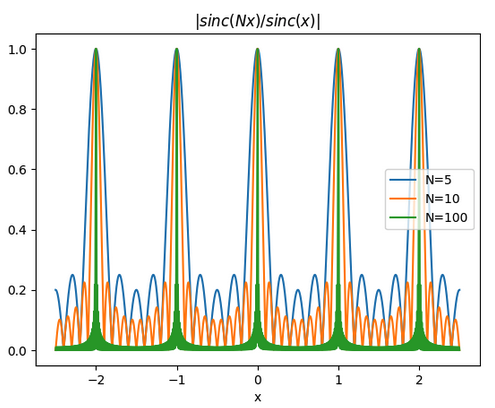
\includegraphics[width=0.4\textwidth]{fig1.png}
\caption{Le module de $\D_N$ pour quelques valeurs de $N$.}
\label{fig-DN}
\end{figure}
%Le lien avec la section précédente peut être fait concernant les équations \ref{eq:hatfdfini} et \ref{eq:fdhatcont} quand on utilise le résultat suivant. Au sens des distributions $\lim_{N\rightarrow\infty}\comb_N=\comb$, donc $\lim_{N\rightarrow\infty}\widehat{\D_N}=\comb$ et l'on peut déduire alors également que $\lim_{N\rightarrow\infty}\D_N=\comb$. Notons au passage que la convolution de $f$ avec le noyau de Dirichlet n'est autre que sa représentation en Série de Fourier.

Maintenant, faisons un peu de comptabilité pour estimer les besoins afin d'obtenir les échantillons de $\hat{F}(u)$ dans le cas d'une grille 2D ($u_k$ de taille $M\times M$) pour  ce placer dans le cadre d'une image:
\begin{enumerate}
\item effectuer la DFT pour obtenir les $N^2$ valeurs $\tilde{a}_{k}$ (ici $k=(k_1,k_2)$), en utilisant un algorithme de type FFT, nécessite typiquement $O(N^2\log N)$ opérations;
\item ensuite pour effectuer 1 convolution (Eq.~\ref{eq:hatfdfini}), il nous faire faire $N^2$ multiplications et $2N$ additions, donc en gros pour obtenir tous les coefficients $\hat{f_d}(u_k)$, il nous faut faire $O((MN)^2)$ opérations;
\item puis il nous faut $O(M^2)$ opérations pour multiplier par les coefficients $\hat{K_x}(u_k)$.
\end{enumerate}
Si on veut terminer la chaîne d'analyse en revenant dans l'espace réel, il nous faut ajouter une DFT inverse qui nécessite $O(M^2\log M)$ opérations. Notons que l'on pourrait également rajouter d'autres tâches pour tenir compte de PSF différentes entre l'image d'origine et l'image finale, et de toutes les transformations (linéaires ou pas) dans l'espace de Fourier pour tenir compte des effets de cisaillement gravitationnel, et autres opérations/transformations géométriques (astronométriques) pour par exemple permettre une co-addition d'images. Cependant, le point critique est le second de la liste ci-dessus.

Si, l'on dispose d'un noyau/interpolant de taille fini qui ne nécessite que $n\leq N$ points en 1D ($n^2$ en 2D) pour remplacer $\D_N$ alors un calcul $O(M^2N^2)$ se réduit à  un calcul $O(n^2 M^2)$, c'est-à-dire qu'on y gagnerait grandement. Le point délicat est comme nous l'avons déjà mentionné, toute approximation de l'interpolateur idéal $\sinc$ dans l'espace réel pour un nombre infini d'échantillons, se paye par des artéfacts qu'il faut pouvoir maitriser.  Le même type de précaution doit être envisagée concernant la version repliée $\D_N$ utilisée dans l'espace de Fourier dans le cas d'un nombre fini ($N$) d'échantillons. Il nous faut donc des conditions de régularités dans l'espace réel et l'espace de Fourier. 
%
\section{Le remplacement du noyau 'idéal' dans l'espace de Fourier}
\label{sec:DNapprox}
%
Comme nous l'avons motivé dans l'introduction, il nous faut dans un premier temps nous focaliser sur l'espace de Fourier. Et comme nous l'avons examiné dans la section précédente, il nous faut obtenir un noyau $K_u$ de taille bien inférieure à $N$, le nombre d'échantillons (1D) de la grille d'origine, qui remplacera le noyau $\D_N$ dans l'équation \ref{eq:hatfdfini} dans le calcul de $\hat{f_d}(u)$. Mais quel est le prix à payer d'utiliser $K_u$ en lieu et place de $\D_N$ qui est le noyau parfait/idéal dans cette opération?

Imaginons une fonction $f(x)$ dont 1 seul échantillon sur les $N$ est non nul: $a_n=1$. Ainsi, 
\begin{equation}
f_d(x) = \delta(x-n) \Rightarrow \hat{f_d}(u) = e^{-2\pi i n u}
\end{equation} 
De plus, les coefficients de la DFT de $f$ satisfont:
\begin{equation}
\forall k\in\Iintv{-N/2,N/2-1},\quad \hat{a}_k = e^{-2\pi i n k/N}
\end{equation}
ce qui peut être vu comme un échantillonnage de la fonction $\hat{f_d}(u)$ au point $u_k=k/N$ d'une grille régulièrement espacée de $1/N$ dans l'intervalle $[-1/2,1/2]$. 

Pour facilité les calculs comme dans le cas du théorème d'échantillonnage, on étend les valeurs de $ \hat{a}_k$ au-delà de l'intervalle $\Iintv{-N/2,N/2-1}$, et en relation avec l'équation \ref{eq:hatfdfini} définissons la fonction
\begin{align}
\hat{s}(u) &= \sum_{k=-\infty}^{\infty} \hat{a}_k K_u(u-k/N) = \sum_k K_u(u-k/N) e^{-2\pi i k n/N}
\label{eq:Su1}
\end{align}
On sait que le théorème d'échantillonnage nous dit qu'avec un échantillonnage de $\Delta=1/N$, alors le filtre/noyau optimal est le sinus cardinal proprement adapté à la taille $\Delta$, soit $\sinc(u/\Delta)=\sinc(Nu)$. \textit{Rq. le filtre $\D_N$ est la version optimale avec des fonctions échantillonnées sur un intervalle fini.}


Ouvrons une parenthèse sous forme d'un petit lemme. 
\begin{lemme}
Soit, la fonction  $h(x)=e^{2\pi i \nu x}$ et un noyau $K$ interpolateur qui définit une approximation $H$ par convolution, alors on a la relation
\begin{align} 
H(x) &= 	h(x) E(\nu,x) &  E(\nu,x)&=\sum_{j=-\infty}^\infty \hat{K}(\nu+j)\  e^{2\pi i jx}
\end{align}
Si de plus l'on exige que $H(0)=h(0)$ alors
\begin{equation}
E(\nu,0)=\sum_{j=-\infty}^\infty \hat{K}(\nu+j) = 1
\label{eq:hatKclosure}
\end{equation}
ce qui fixe également que $H(x)=h(x)$ pour tout $x\in\mathbb{Z}$.
\label{lem:interpSinusoide}
\end{lemme}

La démonstration se sert des éléments de la démonstration du théorème d'échantillonnage (Th.~\ref{th:sampling}).  On peut en effet directement écrire que:
\begin{equation}
H(x) = (K(t)\ast [h(t)\comb(t)])(x) = \sum_{j=-\infty}^\infty h(j) K(x-j)
\end{equation}
qui apparait comme l'interpolation de $h$ avec le noyau $K$. Soit donc $h(t)=e^{2\pi i \nu t}$, la Transformée de Fourier $\hat{H}(u)$ est égale à: 
\begin{align}
\hat{H}(u) &= \hat{K}(u)\times  (\hat{h}\ast \widehat{\comb})(u) \nn \\
&= \hat{K}(u)\times  (\delta(v-\nu)\ast \comb(v))(u) \nn \\
&=   \sum_{j=-\infty}^\infty \hat{K}(u)\ \delta(u-(\nu+j))
\end{align}
En utilisant la TF inverse, il vient alors\footnote{Rq. $\hat{K}(\nu+j)$ est bien la fonction $\hat{K}(u)$ évaluée au point $\nu+j$.}
\begin{align}
H(x) &=  \sum_{j=-\infty}^\infty \int  \hat{K}(u)\ \delta(u-(\nu+j))\ e^{2\pi i xu}du = \sum_{j=-\infty}^\infty \hat{K}(\nu+j)\ e^{2\pi i (\nu+j)x} \nn \\
&= h(x) \sum_{j=-\infty}^\infty \hat{K}(\nu+j)\  e^{2\pi i jx}
\end{align}
C'est bien ce que l'on voulait démontrer. Notons au passage que si $\nu\in [-1/2,1/2]$, on vérifie que $K(x)=\sinc(x)$ est bien l'interpolateur idéal car $\hat{K}(\nu+j)=\boxcar(\nu+j)$ est non nul que ssi $j=0$, ce qui donne $H(x)=h(x)$. En quelque sorte la somme ci-dessus, est une estimation de l'erreur que l'on effectue si on utilise un interpolateur imparfait, d'où la définition de $E(\nu,x)$. Refermons la parenthèse.

Revenons à l'équation \ref{eq:Su1}, si l'on pose $\nu=n/N$ et $x=-Nu$ alors $h(x)=e^{2\pi i \nu x}=\hat{f_d}(u)$, ainsi la fonction d'erreur  $E(\nu,x)$ est égale à 
\begin{align}
E &= \sum_{j=-\infty}^\infty e^{-2\pi i j (-uN)} \widehat{K_u}(n/N-j) \nn\\
&=\widehat{K_u}(n/N)  + \sum_{j\neq 0} \widehat{K_u}(j+n/N) e^{-2\pi i j N u}
\end{align}
or si la contrainte Eq.~\ref{eq:hatKclosure} est satisfaite par le noyau $K_u$, alors
\begin{equation}
\hat{s}(u)= (1-\underbrace{\sum_{j\neq 0} \widehat{K_u}(j+n/N)}_{E_0(n/N)})\hat{f_d}(u) + \sum_{j\neq 0} \widehat{K_u}(j+n/N) e^{-2\pi i j N u} \hat{f_d}(u)
\end{equation}  

En retournant dans l'espace réel par TF inverse, en se rappelant que $f_d(x)=a_n\delta(x-n)$, on obtient alors
\begin{equation}
s(x) = (1-E_0(n/N))\times a_n\delta(x-n) + \sum_{j\neq 0} \widehat{K_u}(j+n/N)\times a_n \delta(x-n-jN)
\label{eq:ghosts}
\end{equation} 
C'est-à-dire qu'au lieu d'avoir $s(x)=a_n\delta(x-n)$, on a
\begin{itemize}
\itemb primo un facteur $1-E_0(n/N)$ qui affecte l'échantillon au point $x=n$, et
\itemb pour chaque point $x=n+jN$ $j\neq 0$, on a une version "fantôme" (\textit{ghost}) de l'échantillon original multiplié par un facteur $\widehat{K_u}(j+n/N)$.
\end{itemize} 
\hfill\\
\begin{figure}[h]
\centering
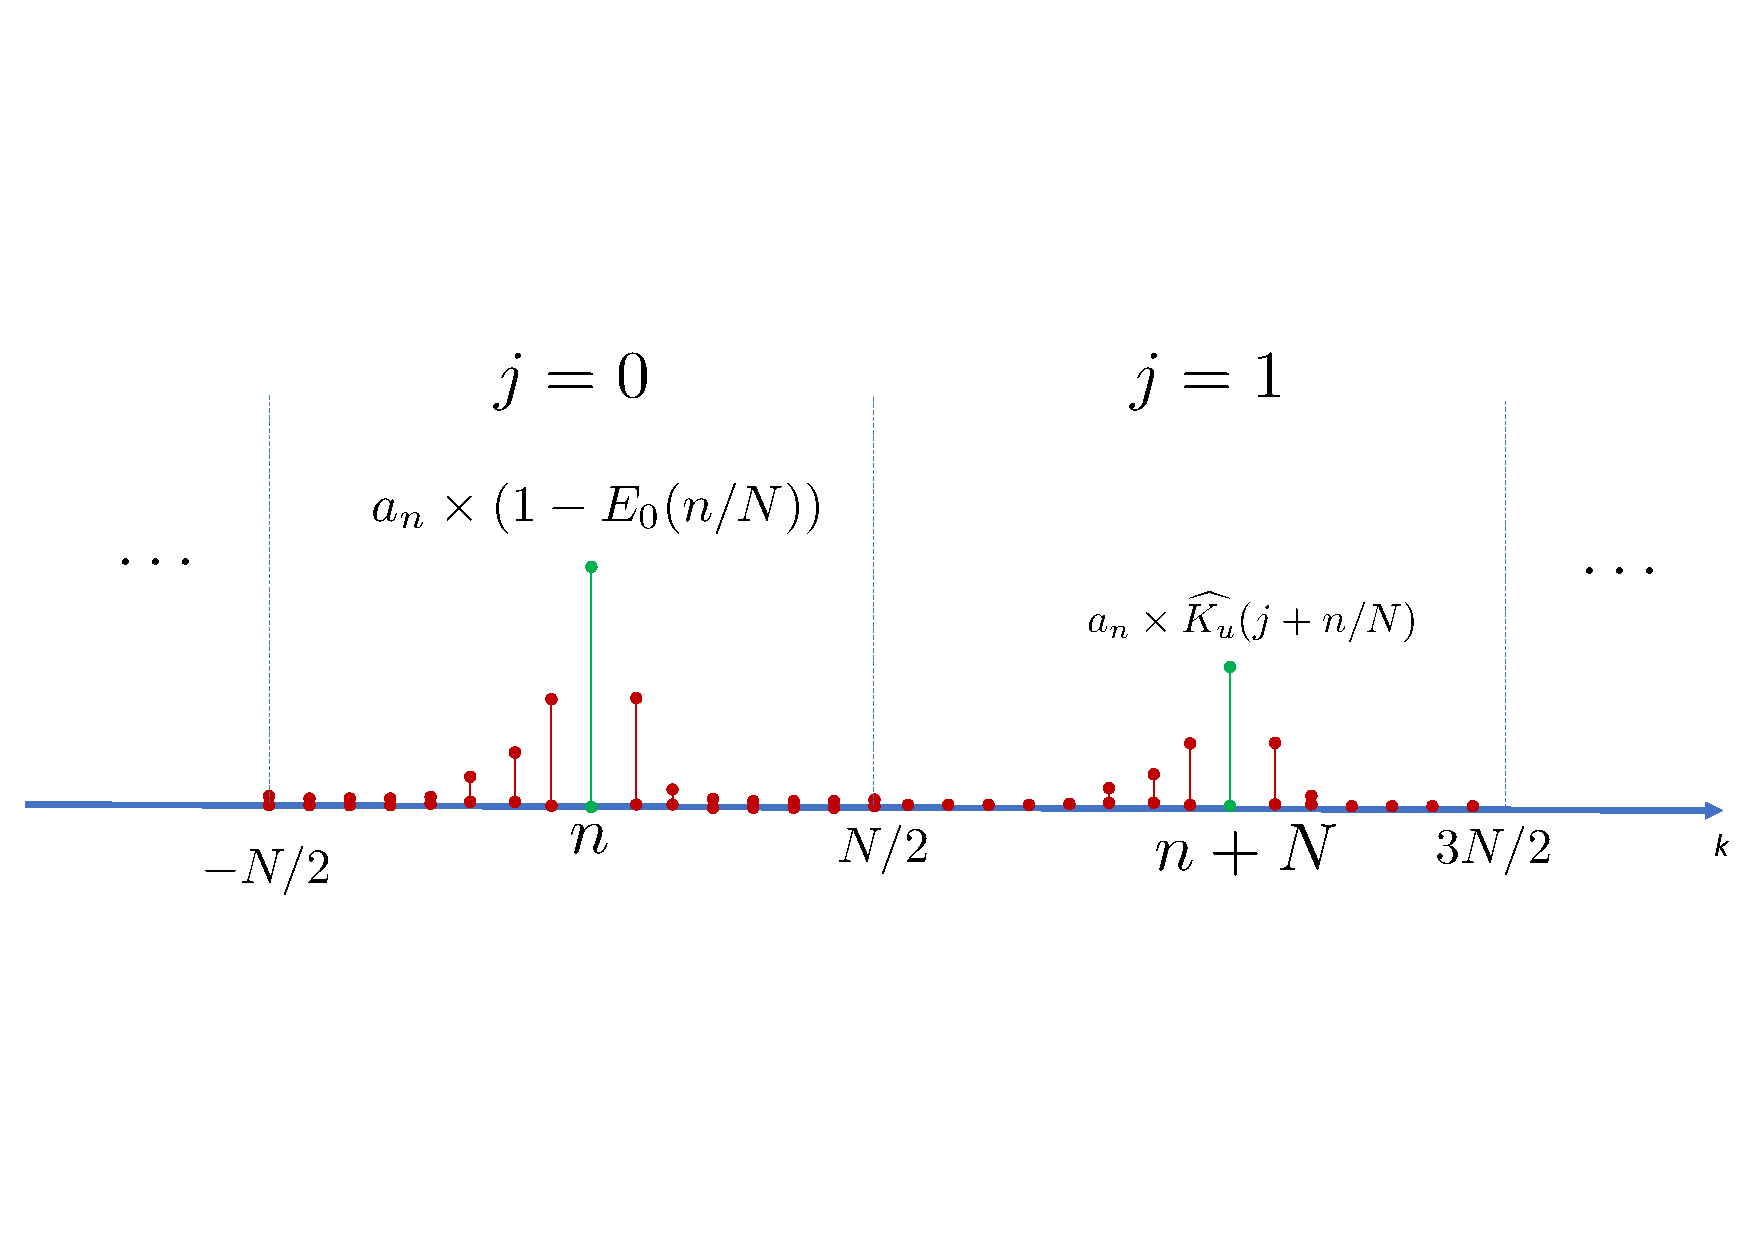
\includegraphics[width=0.8\textwidth]{fig2.pdf}
\caption{Effet d'utiliser un noyau $K_u$ en lieu et place de l'interpolant idéal, sinus cardinal, ou  sinus cardinal périodique.}
\label{fig-Ku-effet}
\end{figure}
Ceci est illustré sur le schéma de la figure \ref{fig-Ku-effet}. Il nous faut donc contrôler ces deux termes. Souvenons-nous que $K_u$ est sensé remplacer $\D_N$ dans l'expression \ref{eq:hatfdfini} sur une plage $u \in [-1/2,1/2]$ ($u$ et la version continu de $u_k=k/N$) et donc $\widehat{K_u}(j+n/N)$ décroit au fur et à mesure que $|j|$ croit. \textbf{Donc les conditions principales concernent les termes  $1-E_0(u)$ et $\widehat{K_u}(u+1)$.}

Nous avons donc deux types de noyau interpolateur en jeu: 
\begin{enumerate}
\item $K_x$ dans l'espace réel (Eq.~\ref{eq:Freal}) qui interpole entre les échantillons $\{i,a_i\}$ ($i\in \Iintv{-N/2,N/2-1}$) pour donner $F(x)$, soit une approximation continue de la fonction $f$ échantillonnée. Si $f$ appartient à une classe de fonctions, type polynôme de degré $d$, on peut trouver $K_x$ qui interpole parfaitement.
\item $K_u$ dans l'espace de Fourier qui remplace le sinus cardinal périodique $\D_N$ (Eq.~\ref{eq:hatfdfini}), qui interpole entre les échantillons $\{k/N, \tilde{a}_k\}$ pour $k\in\Iintv{-N/2,N/2-1}$. Ce remplacement expose à l'apparition de défauts mentionnés ci-dessus.
\end{enumerate}

Avant d'envisager des exemples d'interpolateurs/noyaux, voyons un point qui est nécessaire par exemple pour la famille d'interpolateurs de Lanczos.
%
\section{Propriétés requises des noyaux dans l'espace réel et fond continu}
\label{sec:kernel-freq0}
%
On suppose que le kernel $K_x$ est paire\footnote{Il n'y a pas de raison ici à privilégier des échantillons antérieurs ou postérieurs à un indice $j$.} donc $K_x(-x)=K_x(x)$ ce qui implique que $\hat{K_x}(-u) = \hat{K_x}(-u)$, de plus $K_x(0)=1$ pour assurer $F(j)=f(j)=a_j$, et $K_x(j)=0$ pour $j\neq 0$. Notez également 
\begin{equation}
\forall u, \quad \sum_{j=-\infty}^{\infty} \hat{K_x}(u+j) = 1
\end{equation} 
Cependant, ce n'est pas tout comme l'indique \cite{2014PASP..126..287B}, car au regard du lemme \ref{lem:interpSinusoide}, pour $\nu=0$ alors
\begin{align}
E(0,x) &= \sum_j \hat{K_x}(j) e^{2\pi i j x}
= \hat{K_x}(0) + 2\sum_{j>0}\hat{K_x}(j) \cos(2\pi j x) \nn\\
&= 1+2\sum_{j>0}\hat{K_x}(j)(\cos(2\pi j x)-1)
\end{align}
Par exemple si le terme $\hat{K_x}(1)$ domine alors
\begin{align}
E(0,x) &\approx 1 + 2 \hat{K_x}(1)(\cos(2\pi  x)-1) & 
E^{-1}(0,x) &\approx 1 - 2 \hat{K_x}(1)(\cos(2\pi  x)-1)
\end{align}
On peut opérer alors un changement d'échelle
\begin{align}
\tilde{K}_x(x) &= K_x(x) E^{-1}(0,x) \approx  K_x(x)( 1 - 2 \hat{K_x}(1)(\cos(2\pi  x)-1)) \nn\\
\widehat{\tilde{K}_x}(u) &\approx (1+2\hat{K_x}(1)) \hat{K_x}(u) - \hat{K_x}(1)(\hat{K_x}(u-1)+\hat{K_x}(u+1))
\label{eq:kernel-rescaling}
\end{align}
Notons que $E(0,j)=1$ ($j\in\mathbb{Z}$), donc $\tilde{K}_x(0)=1$ et $\tilde{K}_x(j)=0$ pour $j\neq 0$. On peut également vérifier que $\sum_j \widehat{\tilde{K}_x}(u+j)\approx \sum_j \hat{K_x}(u+j)=1$ par compensation entre les termes. Si de plus, on note formellement une hiérarchie des termes en fonction de puissance d'un paramètre $\varepsilon$ telle que $\hat{K_x}(j)=\varepsilon^j$, alors $\widehat{\tilde{K}_x}(0)= 1+O(\varepsilon^2)$ et $\widehat{\tilde{K}_x}(1)=O(\varepsilon^2)$. 

Ce qui précède a un lien avec la fonction de partition de l'unité d'un noyau.
\begin{propriete}\label{prop:unite}
Soit $K$ un noyau, on dit  qu'il partitionne l'unité si
\begin{equation}
\forall x,\ U(x)\equiv \sum_{j\in\mathbb{Z}} K(x-j) = 1 
\end{equation} 
ce qui a pour conséquence (et vice-versa)
\begin{equation}
\forall u,\ \hat{K}(u) \comb(u)=\delta(u)
\end{equation}
Cette formulation dans l'espace de Fourier donne $\hat{K}(0)=1$ et $\hat{K}(j)=0$ pour tout entier non nul.
\end{propriete} 
On note alors qu'un noyau auquel on procède à la renormalisation par $E(0,x)$ satisfait d'autant mieux cette propriété.
 

Maintenant,  $\widehat{\tilde{K}_x}(u)$ mélange des composantes des  bandes latérales à celles de la bande principale $[-1/2,1/2]$. Plus le coefficient $\hat{K_x}(1)$ est faible plus le mélange est faible. Nous verrons en quoi cela concerne la famille de noyaux de Lanczos et n'affecte pas les autres familles que nous envisageons dans la section suivante.
%
\section{Noyaux pour remplacer le sinus cardinal}
\label{sec:kernel-for-sinuscard-period}
%

\textit{Avertissement: cette section est un peu longue et aurait pu faire par elle-même une note en soi. Je la garde ici par soucis de cohérence. Dans un premier temps, vous pouvez directement aller au "Bilan" (Sec.~\ref{sec:bilan-interpol}).  
}

Je vais passer en revu des noyaux d'interpolation sans pour autant faire une liste exhaustive. Nous allons nous focaliser sur des noyaux en dimension 1, puisque l'extension aux images se fera par produit cartésien (Sec.~\ref{sec:2D}). Je ne considérerai pas pour autant les noyaux de la référence \citep{HU200646} qui utilise des approximations du noyau idéal par fraction continue. Je ne considère pas les noyaux non séparables comme ceux développés par les auteurs de l'article \citep{Shi2006ImageIB}. Pour une "revue", il peut être intéressant de lire \cite{Parsania2016}. Je vais donc plutôt me concentrer sur des noyaux utilisés dans le cadre des librairies pour l'astro comme \textsf{TERAPIX}  et \textsf{SExtractor} \citep{2011ASPC..442..435B} et \textsf{GalSim} \citep{2015A&C....10..121R}. Cependant, je décris les noyaux de type B-Spline et B-Spline \textit{cardinal}, qui sont souvent utilisés dans bien des applications mais qui pour celles qui nous occupent, s'avèreront inadaptés.
%
\subsection{Noyaux de C. Lanczos}
\label{sec:Lanczos}
%
Commençons par la famille des interpolateurs de Cornelius Lanczos (1906-74) \footnote{Son nom a différentes écritures, je prends celle d'un de ces articles. C'est un mathématicien et physicien d'origine hongroise qui a fait des contributions dans ces deux domaines. Il est remarquable que sous la direction de Lipót Fejér, il écrit sa thèse en 1921 "\textit{The functional theoretical relationships of the homogeneous Maxwell equations}" dédiée à Albert Einstein and Max Planck: “\textit{Dedicated to Albert Einstein and Max Planck, the two great standard-bearers of constructive speculation}" \citep{lanczos2004relations}.} utilisés par exemple dans les logiciels: \textsf{SWarp} de la suite \textsf{TERAPIX} \citep{2002ASPC..281..228B}, \textsf{PSFEx} de la suite \textsf{SExtractor} \citep{1996A&AS..117..393B, 2011ASPC..442..435B} et son extension récente \textsf{SourceXtractor++} \citep{2022arXiv221202428K}.

L'idée de C. Lanczos était de régulariser les séries partielles de Fourier qui sont sujettes au phénomène de Gibbs. C'est une famille de noyaux définis par\footnote{Nb. Il y a des erreurs dans l'appendice de l'article \cite{2014PASP..126..287B} qui ont été corrigés dans le code de \textsf{GalSim}.}  
\begin{align}
L_m(x) &= \sinc(x)\sinc(x/m) \boxcar(x/2m) \nn\\
\hat{L}_m(u) &= \frac{1}{2\pi}\Big(
(2mu+m+1)\Si(\pi (2mu+m+1) )- (2mu+m-1)\Si(\pi(2mu+m-1)) \Big. \nn \\
&+\Big. (2mu-m-1)\Si(\pi (2mu-m-1)) - (2mu-m+1)\Si(\pi (2mu-m+1))\Big)
\end{align}
avec  la fonction impaire $\Si(x)$, \textit{sinus intégral}, définie par
\begin{equation}
\Si(x) = \int_0^x \frac{\sin(t)}{t}\ dt
\end{equation}
et $m$ un entier positif typiquement $m\geq3$. Le support du noyau est borné par la contrainte $|x|<m$ ce qui facilite la convolution pour obtenir l'interpolation comme recherché. La figure \ref{fig-Lanczos-kernel} donne quelques exemples d'évolution des graphes de noyaux dans l'espace réel et dans celui de Fourier.
\begin{figure}
\centering
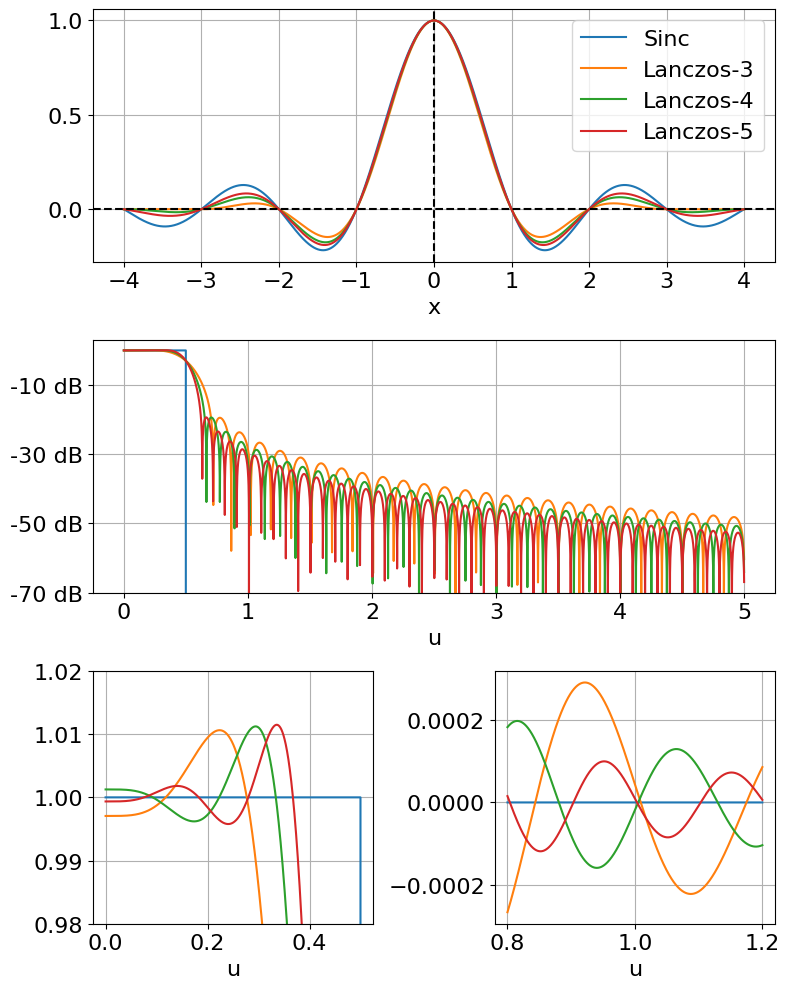
\includegraphics[width=0.8\textwidth]{fig5.png}
\caption{Exemple de noyaux de Lanczos (non normalisé): dans l'espace réel (haut), dans l'espace de Fourier (milieu) avec un zoom aux environs de $u=1$ (bas). Les "dB" sont définis comme l'application de la fonction $10\log_{10}(|v|)$.}
\label{fig-Lanczos-kernel}
\end{figure}
\begin{figure}
\centering
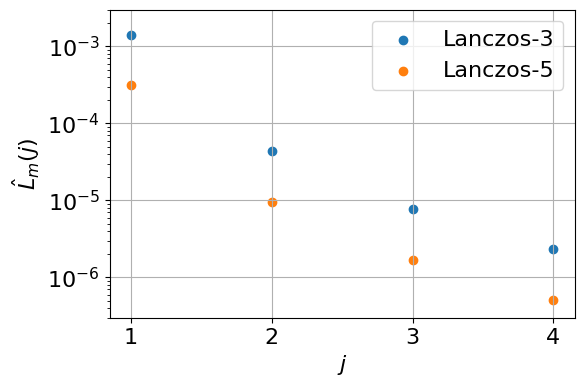
\includegraphics[width=0.6\textwidth]{fig3.png}
\caption{Valeurs de $\hat{L}_m(j)$ pour des entiers $j>0$ et $m=3,4,5$.}
\label{fig-Lanczos-hat-j}
\end{figure}
\begin{figure}
\centering
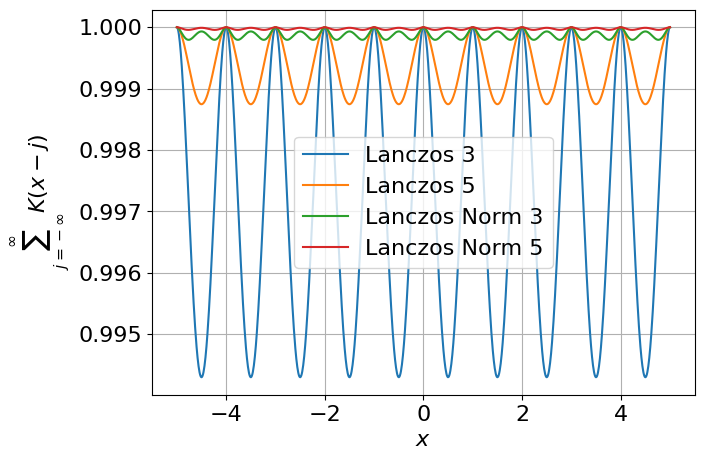
\includegraphics[width=0.6\textwidth]{fig4.png}
\caption{Effet de la procédure de re-normalisation du noyau de Lanczos.}
\label{fig-Lanczos-renorm-closure}
\end{figure}
\begin{figure}
\centering
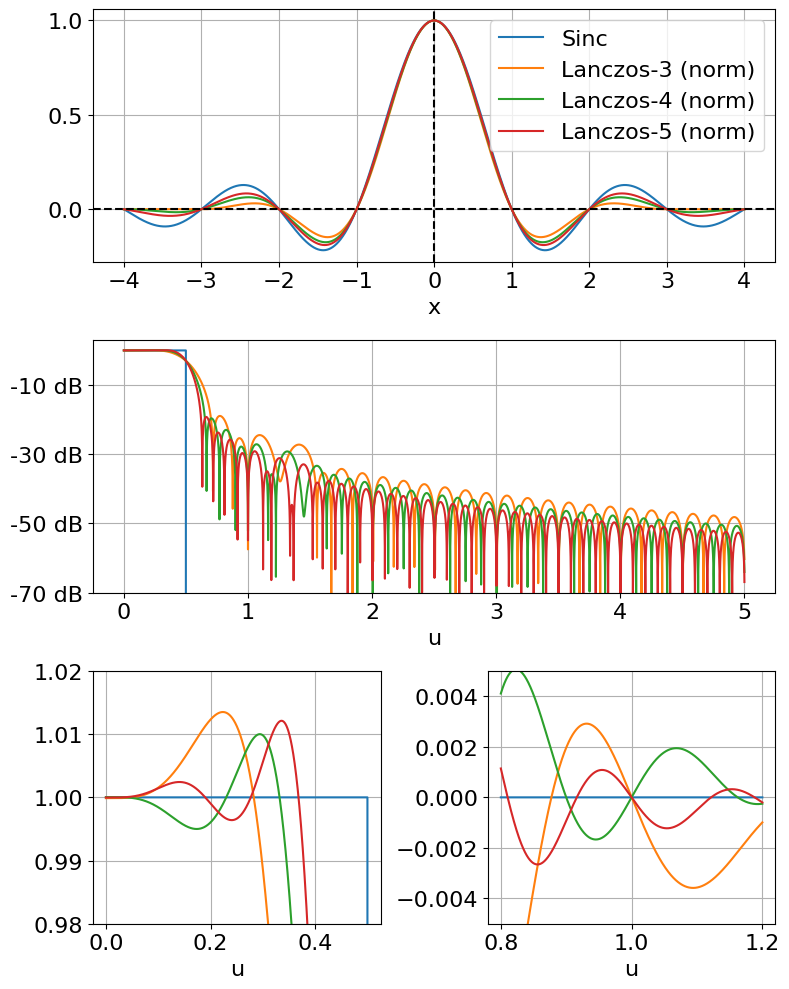
\includegraphics[width=0.8\textwidth]{fig5b.png}
\caption{Mêmes graphiques que sur la figure \ref{fig-Lanczos-kernel} mais effectués avec les noyaux de Lanczos re-normalisés.}
\label{fig-Lanczos-norm-kernel}
\end{figure}

On vérifie facilement que $L_m(0)=1$ et $L_m(i)=0$ pour tout entier non nul. On vérifie également numériquement (à la précision machine) aidé d'un logiciel de calcul formel que ($u\in[-1/2,1/2]$)
\begin{equation}
\lim_{n\rightarrow \infty} \sum_{j=-n}^n \hat{L}_m(u+j)=1
\end{equation}
Cependant $\hat{L}_m(0)\neq 1$ comme par exemple les valeurs pour $m=3,4,5,6$ donnent $0.99705$, $1.00125$, $0.99935$, $1.00037$. Au passage, cela signifie que 
\begin{equation}
\int_{-\infty}^\infty L_m(x)\ dx \neq 1
\end{equation}
De même, on peut constater que $\hat{L}_m(j\neq0)\neq 0$ sur la figure \ref{fig-Lanczos-hat-j}. Ce qui a pour conséquence que le noyau de Lanczos ne partitionne pas l'unité. Il nous faut procéder à un ajustement décrit dans la section \ref{sec:kernel-freq0}. Comme $\hat{L}_m(1)\gg \hat{L}_m(j>1)$ la correction d'ordre 1 de ces formules \ref{eq:kernel-rescaling} suffit à ce stade. L'effet est bien visible sur la figure \ref{fig-Lanczos-renorm-closure}. La déviation maximale de la fonction $U(x)$ (Prop.~\ref{prop:unite})  par rapport à 1, une fois le noyau normalisé est par exemple respectivement de $2\ 10^{-4}$ et $4\ 10^{-5}$ pour $m=3,5$. J'utilise par la suite cette forme renormalisée des noyaux de Lanczos dont les graphes sont donnés sur la figure \ref{fig-Lanczos-norm-kernel}. 

Finalement, un polynôme échantillonné ne peut être interpolé exactement par un noyau de Lanczos (même renormalisé), il n'a pas été construit dans ce but. Dans la suite, nous allons étudier des noyaux  qui ont cette propriété.
%
\subsection{Noyaux polynomiaux par morceaux}
%
Dans cette section, je vais m'intéresser à une classe large de noyaux à support fini constitués de polynômes par morceaux. Les conditions de continuité aux points de $\mathbb{Z}$ constituent des familles de noyaux. 
%
\subsubsection{Famille de noyaux "MZV"}
\label{sec:MZVkernels}
%
Je commence par les noyaux d'écrits dans l'article \cite{Meijering1999}. Ils sont définis de la sorte:
\begin{enumerate}
\item Soit un entier $m>0$, les valeurs du noyau dans l'espace réel sont données par
\begin{equation}
K(x) =\begin{cases}
\sum_{j=0}^n a_{ji} |x|^{j} & i\leq |x| < i+1 \\
0 & |x|\geq m
\end{cases}
\end{equation}
avec  $i\in \Iintv{0,m-1}$. Le degré des polynômes est $n$ sur chaque intervalle $[i,i+1]$.
\item les contraintes imposées sont les suivantes\footnote{$\delta^K_{ij}$ est le symbole de Kronecker valant $1$ si $i=j$, et $0$ sinon.}: d'une part
\begin{align}
&K(j) = \delta^K_{j0},\ \forall j\in \Iintv{0,m-1} \label{eq:Constraints_1}\\
&\lim_{x\rightarrow j^{-}}K^{(\ell)}(x) = \lim_{x\rightarrow j^{+}}K^{(\ell)}(x), \forall j\in \Iintv{0,m} \ \mathrm{et}\ \forall \ell \in  \Iintv{0,L} \label{eq:Constraints_2}
\end{align} 
où $K^{(\ell)}(x)$ est la dérivée d'ordre $\ell$ au point $x$. La première ligne nous est familière, tandis que la seconde concerne la continuité du noyau et de ses dérivées aux points de jointures.
\end{enumerate}
Pour déterminer les $N_{coef}=m(n+1)$ coefficients $\{a_{ji}\}$ il nous faut suffisamment d'équations. La première série de contraintes (Eqs.~\ref{eq:Constraints_1}), nous fixe $m$ équations.  En principe, la seconde série (Eqs.~\ref{eq:Constraints_2}) nous fixerait $(m+1)(L+1)$ équations. Mais de la  continuité en $0$, il est simple de se rendre compte  pour $\ell \in  \Iintv{0,L}$ que $a_{\ell 0}=0$ pour $\ell$ impair, par contre $a_{\ell 0}$ est indéterminé pour $\ell$ pair, il faut donc retirer ces derniers cas du décompte des équations contraignantes. Ainsi, le nombre effectif d'équations est 
\begin{equation}
N_{eq} = m +  (m+1)(L+1) - \ceil{(L+1)/2}
\end{equation}
Faisons un petit test pour se convaincre des choix pris par la suite:
\begin{itemize}
\itemb $n=2m+1$: on peut résoudre les systèmes parfaitement en requérant $L=n-2$.
\itemb $n=2m$: les systèmes peuvent être résolus avec 1 degré de liberté, si $L=n-2$. Pour de plus grandes valeurs de $L$ les systèmes sont sur-contraints.
\itemb $n=2m-1$: pour $m=1$ le système est résoluble parfaitement ($L=0$), tandis que si $m>1$, alors $L=n-2$ les systèmes peuvent être résolus avec 1 degré de liberté, au-delà comme précédemment les systèmes sont sur-contraints.
\itemb $n=2m-2$: soit $L=n-2$ et les systèmes sont résolubles avec 2 degrés de libertés, soit les systèmes sont sur-contraints. 
\end{itemize}
On se rend compte que si l'on fixe la taille du support du noyau ($m$ fixé) alors $n=2m-1$ est la plus petite valeur de $n$ qui permet au mieux de trouver un noyau avec des polynômes dont les coefficients sont connus au plus à 1 coefficient prés, qu'il faut contraindre d'une autre façon que celles déjà examinées. 

Par la suite, pour $m$ fixé, on prend donc $n=2m-1$ et $L=0$ si $m-1$ et il n'y a pas de degré de liberté, sinon $L=n-2$ et il y a 1 degré de liberté. Le noyau est de classe $C^L$ ($C^0$ étant la continuité simple).   

Ainsi, on peut donner l'expression des différents noyaux\footnote{Un script Mathematica permet de trouver les solutions exposés pour n'importe quelle valeur de $m$ (voir Sec.~\ref{sec:MathMZV}).} pour $m=1,2,3$ soit $n=1,3,5$ (noyau linéaire, cubique, et quintique). Les noyaux sont indexés selon le degré $n$ des polynômes.
\begin{itemize}
\item[$\bullet$ \textbf{noyau linéaire}:] ($m=n=1$, $L=0$):
\begin{equation}
K_1(x) = \begin{cases}
1-|x| & |x|< 1 \\
0 & |x| \geq 1
\end{cases}
\label{eq:interp-lineaire}
\end{equation}
En fait c'est la convolution de 2 $\boxcar$: $K_1(x) = (\boxcar \ast \boxcar)(x)$. Sa transformée de Fourier s'écrit donc
\begin{equation}
\hat{K_1}(u) = \sinc^2(u)
\end{equation}
\item[$\bullet$ \textbf{noyau cubique}:]  ($m=2$, $n=3$, $L=1$) posons $a_{31}=c$:
\begin{equation}
K_3(x) = \begin{cases}
1 -(c+3)|x|^2+(2+c)|x|^3 & |x|< 1 \\
-4c + 8x |x|-5c |x|^2+ c |x|^3 & 1\leq |x|<2 \\
0 & |x| \geq 2
\end{cases}
\label{eq:cubic-kernel}
\end{equation}
\item[$\bullet$ \textbf{noyau quintique}:] ($m=3$, $n=5$, $L=3$)  posons $a_{51}=c$:
\begin{equation}
K_5(x) = \begin{cases}
1 +\left(-\frac{5}{2}+8c\right) |x|^2+\left(\frac{45}{16}-18c\right)|x|^4
+ \left(-\frac{21}{16}+10c\right)|x|^5 & |x|< 1 \\
5-66c + 5(-3+53c)|x|+\left(\frac{35}{2}-392c\right)|x|^2 &\\
+(-10+270c)|x|^3+\left(\frac{45}{16}-88c\right)|x|^4+ \left(-\frac{5}{16}+11c\right)|x|^5 & 1\leq |x|<2 \\
-162c + 297 c |x|-216 c|x|^2 + 78 c |x|^3-14 c |x|^4 + c |x|^5 & 2\leq |x|<3\\
0 & |x|\geq 3
\end{cases}
\label{eq:quinticMZV-kernel}
\end{equation}
\end{itemize}
Les expressions générales de $K_n(x)$ et de $\hat{K_n}(u)$ sont telles que $K_n(j)=\hat{K_n}(j)=\delta^K_{0j}$ pour $j\in\mathbb{Z}$. De même, on vérifie que $K_n(x)$ et $\hat{K_n}(u)$ sont des partitions de l'unité.

Maintenant, la question de déterminer $c$ se pose. \cite{Meijering1999} sachant que  $\hat{K_n}^{(1)}(0) = 0$ par symétrie, propose de fixer $\hat{K_n}^{(2)}(0) = 0$. Cela permet de fixer les valeurs: $c=-1/2$ et $c=3/64$ pour $n=3$ et $n=5$. Ainsi, on particularise les expressions données ci-dessus, et on les note $K^{mzv}_n$ (idem pour les TF). Concernant le noyau cubique
\begin{equation}
K^{mzv}_3(x) = \begin{cases}
1 +\frac{1}{2}x^2(3|x|-5) & |x|< 1 \\
-\frac{1}{2}(|x|-1)(|x|-2)^2& 1\leq |x|<2 \\
0 & |x| \geq 2
\end{cases}
\end{equation}
et
\begin{equation}
\widehat{K^{mzv}_3}(u) = \sinc(u)^3 (-2 \cos(\pi u) + 3 \sinc(\pi u))
\end{equation}
 Concernant le noyau quintique
\begin{equation}
K^{mzv}_5(x) = \begin{cases}
1 + x^2\left(-\frac{17}{8}+\frac{x^2}{32}\left(63- 27|x|\right) \right) & |x|< 1 \\
\frac{1}{64}(|x|-1)(|x|-2)(61+|x|(9+|x|(-45+13|x|)))& 1\leq |x|<2 \\
\frac{1}{64}(|x|-2)(|x|-3)^4 & 2\leq |x|<3 \\
0 & |x| \geq 3
\end{cases}
\end{equation}
et
\begin{align}
\widehat{K^{mzv}_5}(u) &=\frac{3}{8} \sinc(u)^3 \Big(35 (\sinc(u) - 
       \cos(\pi u) )/ (\pi^2 u^2) + 
   \sinc(u)^2 (6 \cos(\pi u) - 15 \sinc(u))\Big)
\end{align}
Si $K^{mzv}_3(x)$ est la forme  de noyau cubique utilisé par les auteurs de l'article \cite{2014PASP..126..287B} et le code \textsf{GalSim} il est reconnu comme le \textit{Catmull-Rom cubic interpolation kernel} dans la littérature. 

Ceci dit le choix des valeurs de $c$ proposées par \cite{Meijering1999} pourrait être revu à la lumière de la section \ref{sec:DNapprox} à propos de l'apparition des images fantômes (Eq.~\ref{eq:ghosts}). On pourrait tenter au-delà du fait que $\widehat{K^{mzv}_n}(1)=0$ de contrôler les termes $O(u-1)$. En fait, concernant les noyaux cubique et quintique satisfont:
\begin{align}
\widehat{K^{mzv}_3}(u) &= -3\frac{1+2c}{\pi^2} (u-1) + \frac{12}{\pi^2}(1+2c)(u-1)^2 + O((u-1)^3) \nn\\
\widehat{K^{mzv}_5}(u) &= \frac{45}{8\pi^4}(-3+64c) (u-1) -\frac{135}{4\pi^4}(-3+64c) (u-1)^2 + O((u-1)^3)
\end{align}
Ainsi, les choix $c=(-1/2,3/64)$ permettent non seulement de contrôler les $\widehat{K^{mzv}_n}=1+O(u^4)$ mais aussi $\widehat{K^{mzv}_n}=1+O((u-1)^3)$. Donc nous en resterons là avec cette famille de noyaux. La figure \ref{fig-mzv-kernel} donne les graphes de cette famille de noyaux sur le même modèle que la figure \ref{fig-Lanczos-kernel}. 
\begin{figure}
\centering
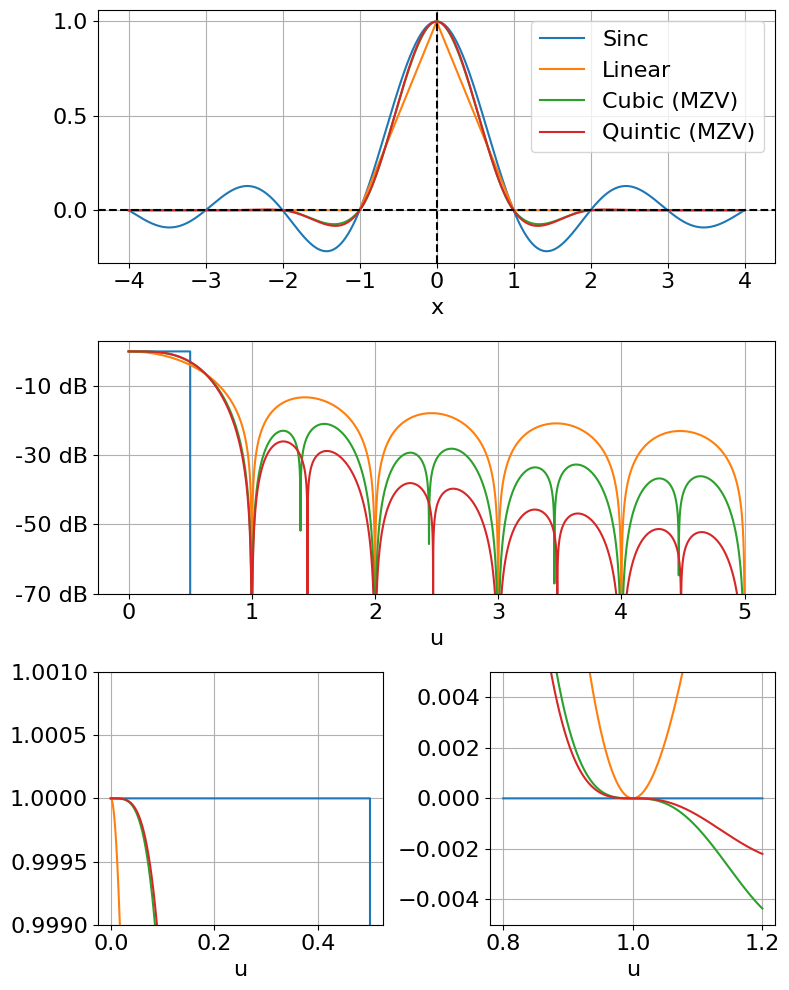
\includegraphics[width=0.8\textwidth]{fig6.png}
\caption{Les noyaux $K_1$, $K^{mzv}_3$ et $K^{mzv}_5$ sur le même modèle que la figure \ref{fig-Lanczos-kernel}.}
\label{fig-mzv-kernel}
\end{figure}
%
\subsubsection{Famille de noyaux "BG" dont une variante quintique}
\label{sec:BGKernels}
% 
\cite{2014PASP..126..287B} proposent dans leur article non pas une famille en tant que telle, car ils se focalisent sur un noyau quintique, mais on peut retrouver dans un même schéma, le noyau cubique de $K^{mzv}_3(x)$ autrement appelé le noyau de Catmull-Rom,  la version "BG" de noyau quintique ainsi qu'une variante, elle-même différente de $K^{mzv}_5(x)$.

Pour cela, on utilise la même définition des noyaux MZV ainsi que les même notations, notamment le paramètre $m$ donne non seulement la taille du support du noyau, et aussi le degré des polynômes $n=2m-1$. Il y a donc $2m^2$ coefficients à déterminer\footnote{Un script Mathematica permet de trouver les solutions pour le noyau cubique, la famille de noyaux quintiques, et pour un noyau spetique non exposé (voir Sec.~\ref{sec:MathBG}).}. Les contraintes imposées sont les suivantes:
\begin{itemize}
\itemb on commence par série des contraintes identiques Eqs.~\ref{eq:Constraints_1}:
\begin{align}
K(j) = \delta^K_{j0},\ \forall j\in \Iintv{0,m-1} \label{eq:ConstBG_1}
\end{align} 
\itemb ensuite, on limite la régularité du noyau par rapport au noyau MZV dans l'espace réel par requérir
\begin{align}
& a_{\ell,0}=0, \quad \ell \in  \Iintv{1,m-1}\ \mathrm{et} \ \ell \ \mathrm{impair};
\end{align}
et pour $m\geq3$
\begin{align}
&\lim_{x\rightarrow j^{-}}K^{(\ell)}(x) = \lim_{x\rightarrow j^{+}}K^{(\ell)}(x), \forall j\in \Iintv{1,m} \ \mathrm{et}\ \forall \ell \in  \Iintv{0,n-4} \label{eq:ConstBG_2}
\end{align}
\itemb par contre dans l'espace de Fourier, nous imposons
\begin{align}
& \widehat{K}(0)=1 \\
&\reallywidehat{K^{(\ell)}}(0) = 0, \forall \ell\in \Iintv{2,n} \ \mathrm{et}\ \ \ell \ \mathrm{pair} \\
& \reallywidehat{K^{(\ell)}}(1) = 0, \forall \ell\in \Iintv{0,n-1}
\end{align}
\end{itemize}
Pour $m=2$ ($n=3$), on retrouve le noyau cubique de la section précédente. Concernant $m=3$ ($n=5)$, les coefficients $\{a_{ji}\}$ sont tous déterminés sauf 1 que l'on peut choisir $a_{20}$. On peut alors avoir plusieurs choix pour déterminer cette dernière inconnue.

Soit on fixe $a_{20}=0$, ce qui donne la forme de noyau quintique de l'article \cite{2014PASP..126..287B} à savoir\footnote{Nb. l'expression dans l'article n'est pas correcte puisqu'il faut assurer que $K(-x)=K(x)$, c'est-à-dire qu'il faut faire apparaître les valeurs absolues. Le code de \textsf{GalSim} utilise la bonne formulation. De plus, je donne ici la TF du noyau.}
\begin{align}
K^{bg}_5(x) &= \begin{cases}
1 + \frac{1}{12}|x|^3 \Big(-95+|x|(138-55|x|)\Big) & |x|< 1 \\
\frac{1}{24}(|x|-1)(|x|-2)\Big(-138+|x|(348+|x|(-249+55|x|))\Big)& 1\leq |x|<2 \\
-\frac{1}{24}(|x|-2)(|x|-3)^2\Big(54+|x|(-50+11|x|)\Big) & 2\leq |x|<3 \nn \\
0 & |x| \geq 3
\end{cases}\\
\widehat{K^{bg}_5}(u)&=\sinc(u)^5 \Big(2(-27+(\pi u)^2)\cos(\pi u)+\sinc(u)(55-19(\pi u)^2)\Big)
\label{eq:quinticBG-kernel}
\end{align}
Les dérivées secondes de ce noyaux sont discontinues aux points de jonction $K^{bg}_5(j)$ ($j=1,2,3$). Concernant la régularité de $\widehat{K^{bg}_5}(u)$, nous avons\footnote{Nb. attention $O(x^n)$ est bien "d'ordre de $x^n$" qui n'est pas à confondre avec $o(x^n)$ qui est l'indication de "négligeable par rapport à $x^n$).} $\widehat{K^{bg}_5}(u)=O(u^6)$ et $\widehat{K^{bg}_5}(u-j)=O((u-j)^5)$ pour ($j=1,2,3$). 

C'est là, où j'ai utilisé la liberté du choix de la valeur de $a_{20}$ pour faire écho à la lumière de l'équation \ref{eq:ghosts} de la section \ref{sec:DNapprox} afin de diminuer l'influence des images fantômes. On peut choisir $a_{20}$ de telle façon que $\widehat{K_5}(1)=O((u-1)^6)$ ce qui donne
\begin{equation}
a_{20} = -\frac{5}{4}\left(\frac{27-\pi^2}{15-\pi^2}\right)
\end{equation}
Ainsi
\begin{align}
K^{je}_5(x) &= \begin{cases}
\frac{1}{12} \Big((138-55 |x|) |x|-95\Big) |x|^3+\frac{5 \left(\pi ^2-27\right)}{4 \left(\pi^2-15\right)} (|x|-1)^2 (2 |x|-1) x^2 +1& |x|< 1 \\
\frac{1}{24 \left(\pi^2-15\right)}(|x|-2) (|x|-1) \Big(\pi ^2 (|x| (|x| (25 |x|-114)+153)-48)\Big.& \nn\\
\qquad\qquad \Big.-15 (|x| ((|x|-6) |x|-3)+24)\Big)& 1\leq |x|<2 \nn\\
-\frac{1}{24 \left(\pi ^2-15\right)}(|x|-3)^2 (|x|-2) \Big(\pi^2 (|x|-3) (5 |x|-8)-3 (|x|-7) |x|\Big) & 2\leq |x|<3 \nn \\
0 & |x| \geq 3
\end{cases}\\
\widehat{K^{je}_5}(u)&= \frac{\sinc(\pi u)^5}{\pi^2-15} \left(24 \pi^2 (u^2-1) \cos (\pi u)-(\pi^2 ((39+7 \pi^2) u^2-25)+15) \sinc(\pi  u)\right)
\label{eq:quinticJE-kernel}
\end{align}
$K^{je}_5(j)$ a toutes les dérivées secondes discontinues en $j=0,\dots,3$, tandis qu'en même temps  $\widehat{K^{je}_5}(u)=O((u-j)^6)$ (cf. pas uniquement en $j=0,1$). On vérifie aussi que pour toutes les valeurs de $a_{20}$ à la fois $K_5$ et $\widehat{K_5}$ sont des partitions de l'unité.

La figure \ref{fig-quintic-kernels} présente les différents noyaux quintiques: $K^{mzv}_5$, $K^{bg}_5$ et $K^{je}_5$. 
\begin{figure}
\centering
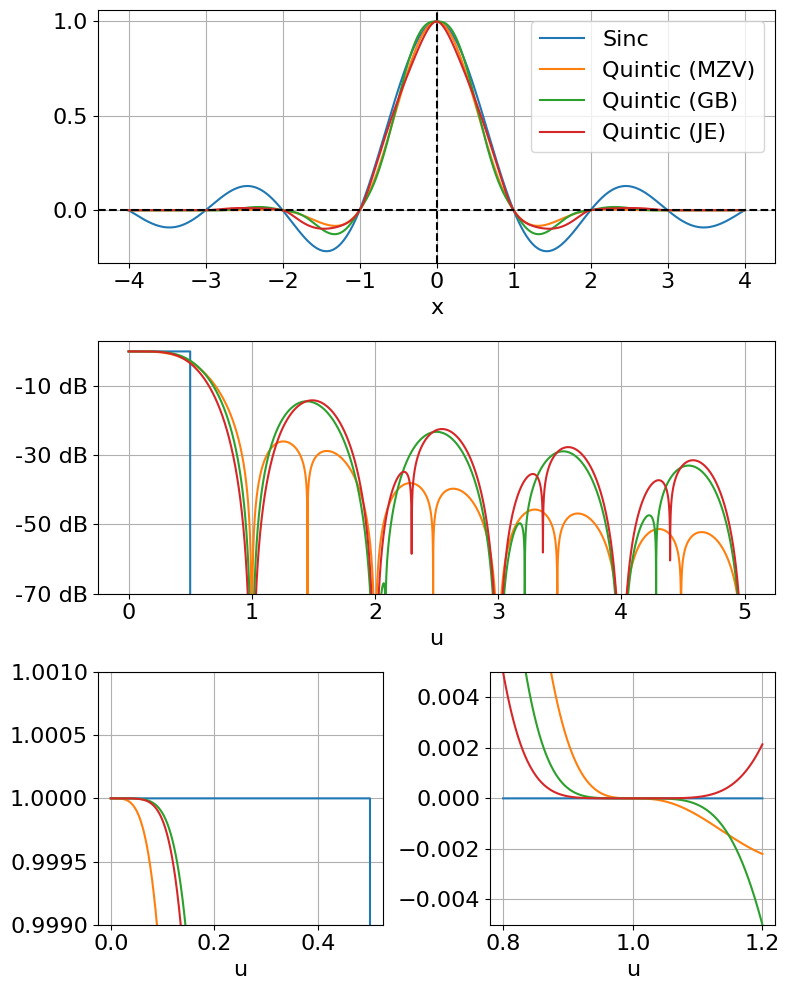
\includegraphics[width=0.8\textwidth]{fig10.png}
\caption{Les noyaux de type "quintique": $K^{mzv}_5$, $K^{bg}_5$ et $K^{je}_5$  sur le même modèle que la figure \ref{fig-Lanczos-kernel}.}
\label{fig-quintic-kernels}
\end{figure}

%
\subsubsection{Famille de noyaux : B-spline (cardinale)}
%
Les \textit{splines} sont très utilisés (math/ingénierie) et je ne peux ouvrir l'ensemble des applications. Concernant l'interpolation, on les présente souvent dans l'espace réel, afin de concevoir une représentation par exemple cubique par morceaux, entres les noeuds dont on connait la position dans un espace multi-dimensionnel. Concernant la possibilité d'obtenir une base orthogonale, on exploite ce que l'on nomme soit les \textit{box splines} \cite{10.5555/1525499}, soit les \textit{B-splines} et les versions "cardinal" \cite{Unser1993a} que nous allons manipuler.  Dans la suite, je vais me concentrer sur un cas particulier pour comparaison avec les sections précédentes. 

En fait l'idée est la suivante. Dans le domaine de Fourier, l'expression du noyau d'une B-spline est la suivante\footnote{Nb. il peut y avoir différentes formulations non seulement via les conventions de la transformée de Fourier, mais aussi si on considère des B-splines centrées ou non.}
\begin{equation}
\hat{\beta}_m(u) = \sinc(u)^{m+1}
\end{equation}
ce qui dans l'espace réel donne $m$ convolutions de la fonction $\boxcar(x)$:
\begin{equation}
\beta_m(x) = (\underbrace{\boxcar \ast \dots \ast \boxcar}_{(m+1)\mathrm{-fois}})(x)
\end{equation}
Un exemple est donné sur la figure \ref{fig-Bspline3-kernel} pour le $m=3$ que nous allons détaillé. L'expression dans l'espace réel peut se mettre sous la forme de polynôme d'ordre $m$ par morceaux qui pour $\beta_3$ donne une formulation "cubique":
\begin{equation}
\beta_3(x) = \begin{cases}
\frac{2}{3}+\frac{1}{2} x^2(|x|-2) & |x|< 1 \\
-\frac{1}{6} (|x|-2)^3 & 1\leq |x|<2 \\
0 & |x| \geq 2
\end{cases}
\end{equation}
Si $\beta_3(x)$ est une partition de l'unité (en particulier $\sum_{j=-1}^1 \beta_3(j)=1$), par contre $\beta_3(0)\neq 1$  et $\beta_3(1)\neq 0$. De même, si $\hat{\beta}_3(0)=1$ et $\hat{\beta}_3(1)=0$ par contre  $\hat{\beta}(u)$ n'est pas une partition de l'unité (voir Fig.~\ref{fig-UnityBspline3}).
%
\begin{figure}
\centering
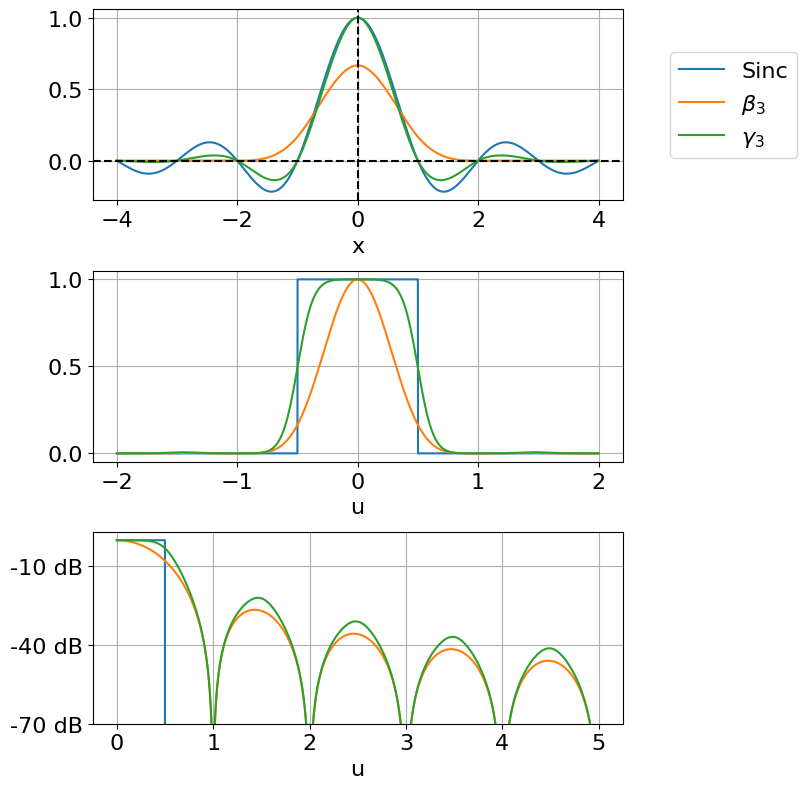
\includegraphics[width=0.6\textwidth]{fig7.png}
\caption{Graphes de la B-spline $\beta_3$ et de sa version "cardinal" $\gamma_3$ comparés à celui du sinus cardinal.}
\label{fig-Bspline3-kernel}
\end{figure}
%
\begin{figure}
\centering
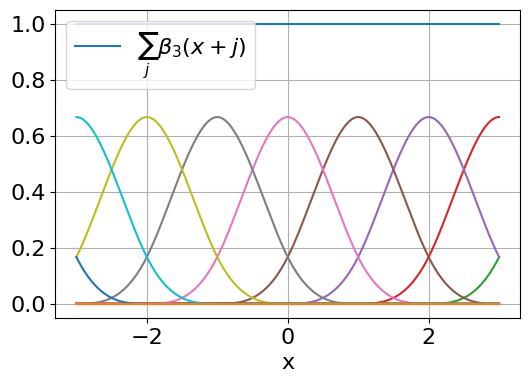
\includegraphics[width=0.4\textwidth]{fig8a.png}
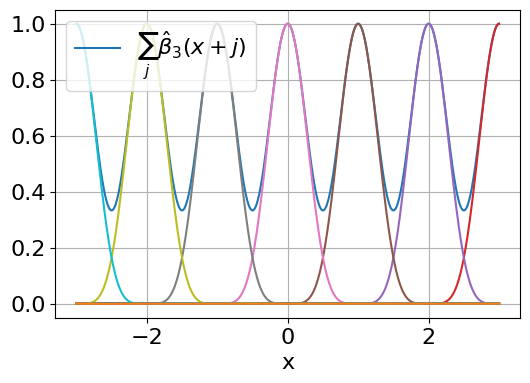
\includegraphics[width=0.4\textwidth]{fig8b.png}
\caption{La B-spline $\beta_3$ partitionne l'unité dans l'espace réel, ce n'est pas le cas de $\hat{\beta}_3$ dans l'espace de Fourier.}
\label{fig-UnityBspline3}
\end{figure}
%

Remarquons que l'interpolation linéaire ($\beta_1$) (Eq.~\ref{eq:interp-lineaire}) est la convolution de deux $\boxcar$ et qu'il n'a pas les défauts mis en évidence ci-dessus de $\beta_3$. En fait, le noyau linéaire a été "flouté" (\textit{blur kernel}). C'est ce qu'il faut corriger, et c'est le sujet des \textit{cardinal B-splines}.

Le noyau de floutage qui affecte $\beta_3$ est 
\begin{equation}
b_3(x) = \sum_{j=-1}^1 \beta_3(j)\delta(x-j)
\end{equation}
avec $\beta_3(j)=\{1/6,2/3,1/6\}$ pour respectivement $j=\{-1,0,1\}$. La transformée de Fourier inverse fournit la représentation suivante:
\begin{equation}
\hat{b}_3(u)= \frac{2}{3} + 2\frac{1}{6}\cos(2\pi u) = 1-\frac{2}{3}\sin(\pi u)^2
\end{equation}
La première forme est généralisable (voir Eq. 3.22 de \cite{Unser1993a}) et il n'est pas fortuit de trouver les coefficients $\beta_3(0)$ et $\beta_3(1)$. La seconde forme permet un usage pratique  utilisée ci-dessous. Donc, si l'on veut déconvoluer le "flou", il suffit alors de définir 
\begin{equation}
\hat{\gamma}_3(u) = \hat{\beta}_3(u)\times \hat{b}^{-1}_3(u) = \frac{\sinc^4(u)}{1-\frac{2}{3}\sin(\pi u)^2}
\label{eq:hatgam3}
\end{equation}  
où $\hat{b}^{-1}_3(u)$ est en termes de traitement du signal \textit{la réponse impulsionnelle du filtre B-spline}.

L'inversion dans le cas $m=3$ se fait en utilisant la relation du binôme de $(1-x)^{-1}$ qui fait apparaitre les facteurs  $\sin(\pi u)^{2n}$ qui se décompose\footnote{\url{https://en.wikipedia.org/wiki/List_of_trigonometric_identities}} selon
\begin{equation}
\sin(\pi u)^{2n} = \frac{1}{2^{2n}}\binom{2n}{n}+\frac{(-1)^n}{2^{2n-1}}\sum_{k=0}^{n-1} (-1)^k \binom{2n}{k}\cos(2(n-k)\pi u)
\end{equation}
Puis, en utilisant le fait que 
\begin{equation}
\cos(2(n-k)\pi u) \xrightarrow[]{TF^{-1}} \frac{1}{2}(\delta(x-(n-k))+\delta(x+(n-k)))
\end{equation}
on peut alors mettre $b^{-1}_3(x)$ sous la forme
\begin{equation}
b^{-1}_3(x) = \sum_{n=-\infty}^\infty s_3(n) \delta(x-n)
\end{equation}
avec\footnote{nb. Mathematica aide bien pour trouver la forme compacte.}
\begin{equation}
s_3(n) = (-1)^n \sum_{k=0}^\infty \frac{1}{6^{|n|+k}} \binom{2(|n|+k)}{k} =  \frac{(-1)^n\sqrt{3}}{(2+\sqrt{3})^{|n|}}
\end{equation}
Remarquons au passage la propriété:
\begin{equation}
\sum_{n=-\infty}^\infty s_3(n) = 1
\end{equation} 
Finalement, l'expression de $\gamma_3(x)$  est donnée par convolution
\begin{equation}
\gamma_3(x) = (\beta_3 \ast b^{-1}_3)(x) =  \sum_{n=-\infty}^\infty s_3(n) \beta_3(x-n)
\label{eq:gam3}
\end{equation}
La parité de $\gamma_3$ et la même que celle de $\beta_3$. Notons qu'étant donné que $\beta_3(j)\neq 0$ pour $j=\{-1,0,1\}$ et $\beta_3(x)$ est paire ainsi que $s_3(n)$ nous avons
\begin{align}
\gamma_3(0) &=\sum_{n=-\infty}^\infty s_3(n) \beta_3(n)
= \left\{-\frac{\sqrt{3}}{2+\sqrt{3}},\sqrt{3},-\frac{\sqrt{3}}{2+\sqrt{3}}\right\}.\left\{\frac{1}{6},\frac{2}{3},\frac{1}{6}\right\} = 1
\label{eq:gamma30}
\end{align}
De plus si l'on note $s_3(n)=(-1)^n\sqrt{3}a^{|n|}$ avec $a=(2+\sqrt{3})^{-1}=2-\sqrt{3}$, alors pour $j\geq 1$ nous avons
\begin{align}
\gamma_3(j) &= s_3(j)\beta_3(0) + \beta_3(1)[s_3(j-1)+s_3(j+1)]\nn \\
&= \sqrt{3} (-1)^j a^j (\beta_3(0)-\beta_3(1)(1/a+a)) = 0
\end{align}
(et par symétrie $\gamma_3(-j)=0$).  

Les graphes de $\gamma_3(x)$ et $\hat{\gamma}_3(u)$ comparés à ceux de $\beta_3(x)$ et $\hat{\beta}_3(u)$ sont montrés sur la figure \ref{fig-Bspline3-kernel}. Maintenant, la figure \ref{fig-UnityBsplineCard3} apporte la touche finale en montrant que la B-Spline cardiale partitionne bien l'unité à la fois dans l'espace réel mais aussi dans l'espace de Fourier. Ces propriétés sont aisément démontrables en utilisant, concernant l'espace réel, le fait que $\beta_3(x)$ partitionne l'unité  et que la somme des $s_3(n)$ donne aussi l'unité, et concernant l'espace de Fourier on rappelle que $\hat{\gamma}_3(u)$ a été conçue pour réaliser la propriété de partitionnement. Les développements ci-dessus détaillés pour $\gamma_3$ sont généralisables pour $m$ quelconque, voir par exemple voir \cite{Unser1993a}.
\begin{figure}
\centering
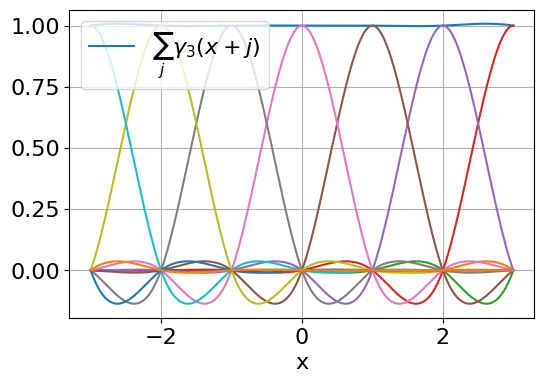
\includegraphics[width=0.4\textwidth]{fig9a.png}
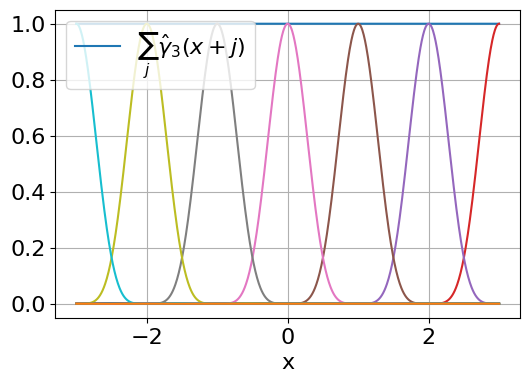
\includegraphics[width=0.4\textwidth]{fig9b.png}
\caption{La B-spline \textit{cardinal} $\gamma_3$ partitionne l'unité dans l'espace réel, et il en est de même dans l'espace de Fourier pour $\hat{\gamma}_3$ ce qui contraste avec le figure \ref{fig-UnityBspline3}.}
\label{fig-UnityBsplineCard3}
\end{figure}

Maintenant, le hic avec $\gamma_3(x)$ qui pourrait être utilisé pour remplacer le sinus cardinal dans notre application (Sec.~\ref{sec:DNapprox}), c'est son support. En principe, il est de taille infini. 
%On peut certes tenter une approximation en utilisant une partie des coefficients $s_3(n)$, mais la figure \ref{fig-cubic-kernels-x-support} permet de comparer le support de différents noyaux "cubiques". On se rend compte que si le support de $\beta_3$ est $[-2,2]$, le support d'une approximation  de $\gamma_3(x)$ devrait être au minimum $[-3,3]$ voire $[-4,4]$. En comparaison les noyaux quintiques "MZV" (Eq.~\ref{eq:quinticMZV-kernel}), "BG" (Eq.~\ref{eq:quinticBG-kernel}) et "JE" (Eq.~\ref{eq:quinticJE-kernel}) ont un support $[-3,3]$, et un B-Spline cardinal quintique serait encore plus important. 
%\begin{figure}
%\centering
%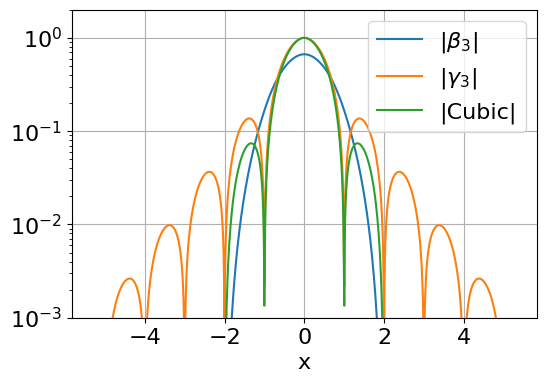
\includegraphics[width=0.4\textwidth]{fig11.png}
%\caption{Comparaison de $|\beta_3(x)|$, $|\gamma_3(x)|$ et du noyau cubique (ex. celui de "MZV" (Eq.~\ref{eq:cubic-kernel}). Un noyau "quintique" de a un support $[-3,3]$.}
%\label{fig-cubic-kernels-x-support}
%\end{figure}
Or, nous avons motivé (Sec.~\ref{sec:interpFinite}) le fait de choisir des noyaux dont la taille de support est le plus petit possible (intervenant au carré) moyennant des qualités pour réduire les images fantômes.  On peut tenter de procéder à une approximation qui permettrait de réduire le support de $\gamma_m(x)$. Mais on va tout de même avoir un problème.

On peut se faire une idée du problème, en se posant la question de trouver les coefficients $s_3(n)$ autrement que la démarche entreprise ci-dessus. Je vais suivre la démarche\footnote{nb. L'article non publié de l'auteur est très pédagogique, tourné pour des applications Web de type Facebook, Instagram même s'il mentionne que ces approximations devrait être revues pour des applications plus demandeuses de précisions. C'est ce que l'on constate d'ailleurs. C'est assez original que l'auteur n'est pas remarqué qu'il (re)construisait les B-Splines, et que ses "Magic Kernel(s) Sharp" sont les B-Splines cardinal.} de \cite{Costella2021} en adaptant les notations. En fait, rappelons que pour la version "cardinale" $\gamma_3(n)=0$ pour $|n|\geq 1$ et que cela est généralisable pour d'autres valeurs de $m$. Une approximation d'ordre $o$ consiste alors à requérir que $\gamma^{(o)}_3(n)=0$ pour $1\leq n\leq o$. Dans la suite on se limite aux  B-Splines tels que $\beta_m(n\geq 3)=0$. Les coefficients $S=\{s_m(n)\}_{1\geq n}$ (sachant que $s_m(-n)=s_m(n)$ et $\sum_{n=-\infty}^\infty s_m(n)=1$ ce qui donne $s_m(0)$) sont alors solutions d'un système linéaire dont la forme (indexation commençant à 1) est la suivante:
\begin{equation}
(A+Z-2B^T R)S+B^T = 0
\end{equation}
 Les matrices s'écrivent comme suit\footnote{$0_{n,n}$ et $1_{n,n}$ représentent respectivement la matrice nulle et la matrice identité de taille $n\times n$.} 
\begin{equation}
A= \begin{bmatrix}
\beta_0 & \beta_1&\beta_2 & 0 & 0 & 0 & 0 & 0 &\ldots\\
\beta_1 & \beta_0 & \beta_1&\beta_2 & 0 & 0 &0 & 0 &\ldots \\
\beta_2 & \beta_1 & \beta_0 & \beta_1&\beta_2 & 0 & 0&0 & \ldots\\
0 & \beta_2 & \beta_1 & \beta_0 & \beta_1&\beta_2 & 0 &0& \ldots\\
0& 0 & \beta_2 & \beta_1 & \beta_0 & \beta_1&\beta_2 & 0 & \ldots\\
\vdots & \vdots & \vdots  & \vdots & \vdots &\vdots & \vdots & \ddots
\end{bmatrix}
\end{equation}
\begin{equation}
Z = 0\ \mathrm{sauf}\  Z(1,1)=\beta_2
\end{equation}
\begin{equation}
B = (\beta_1,\beta_2,0,\ldots), \quad R=(1,1,\ldots)
\end{equation}
La solution d'ordre $o$ tronque les matrices pour n'avoir que $o$ lignes ou colonnes. Cela donne par exemple les solutions disposées dans la table \ref{tab-scoeff-bsplinecardapprox}.
\begin{table}
\small
\centering
\begin{tabular}{cc|*{20}{c}}
\toprule
 $m$ & $o$ & $s_m(\pm 1)$ & $s_m(\pm 2)$ & $s_m(\pm 3)$ & $s_m(\pm 4)$ & $\ldots$& \\ \midrule
   3 & 1   & $-\frac{1}{2}$ &       & \\
   . & 3   &  $-\frac{15}{32}$&$\frac{1}{8}$&$-\frac{1}{32}$&   \\
   . & 5   &  $-\frac{209}{450}$& $\frac{28}{225}$ & $-\frac{1}{30}$  & $\frac{2}{225}$&$-\frac{1}{450}$& \\ \midrule
   5 & 1   & $-\frac{26}{15}$& \\
   . & 3   & $-\frac{3133}{2200}$&$\frac{13173}{22000}$&$-\frac{884}{4125}$ & \\
   . & 8   & $-1.32017$ & $0.57265$& $-0.24674$& $0.10623$& $-0.04569$& $0.01956$& 
$-0.00816$& $0.00292$ \\
\bottomrule
\end{tabular}
\caption{Exemples de listes de coefficients $s_m$ pour différentes ordres d'approximation $o$ concernant les BSplines $\gamma^{(o)}_3$ et $\gamma^{(o)}_5$.} 
\label{tab-scoeff-bsplinecardapprox}
\end{table}
Une fois les valeurs de $\{s^{(o)}_m(n)\}_{1\leq n\leq o+1}$ obtenues, alors $\gamma_m^{(o)}(x)$ est le résultat d'une convolution de type Eq.~\ref{eq:gam3} où l'on remplace la séquence des $\{s_m(n)\}$. On peut apprécier la convergence de $\gamma^{(o)}_3$ vers $\gamma_3$ tant dans l'espace réel (Fig.~\ref{fig-gamma3-approx-real}) que dans l'espace de Fourier (Fig.~\ref{fig-gamma3-approx-fourier}). La partition de l'unité dans l'espace de Fourier n'est pas assurée parfaitement à cause des oscillations non compensées dans la première zone de Nyquist, comme on peut le voir sur la figure  \ref{fig-gamma3-approx-unite-fourier}, mais cela reste dans l'ordre de grandeur de $0.001$.
\begin{figure}
\centering
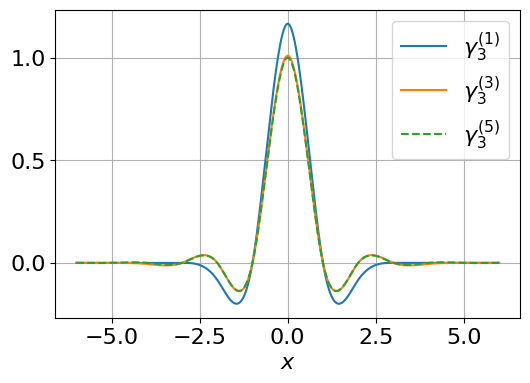
\includegraphics[width=0.4\textwidth]{fig13a.png}
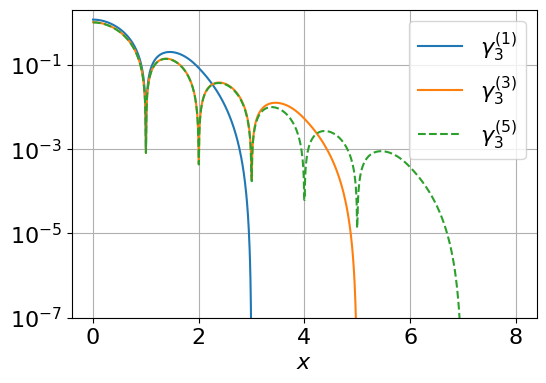
\includegraphics[width=0.4\textwidth]{fig13b.png}
\caption{Quelques graphes concernant les approximations de $\gamma_3$ dans l'espace réel.}
\label{fig-gamma3-approx-real}
\end{figure}
\begin{figure}
\centering
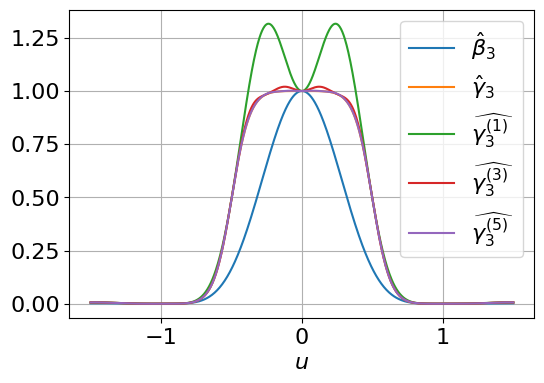
\includegraphics[width=0.4\textwidth]{fig14a.png}
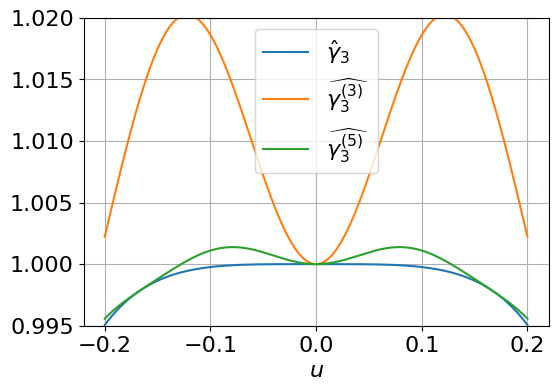
\includegraphics[width=0.4\textwidth]{fig14b.png}
\caption{Quelques graphes concernant les approximations de $\gamma_3$ dans l'espace de Fourier.}
\label{fig-gamma3-approx-fourier}
\end{figure}


\begin{figure}
\centering
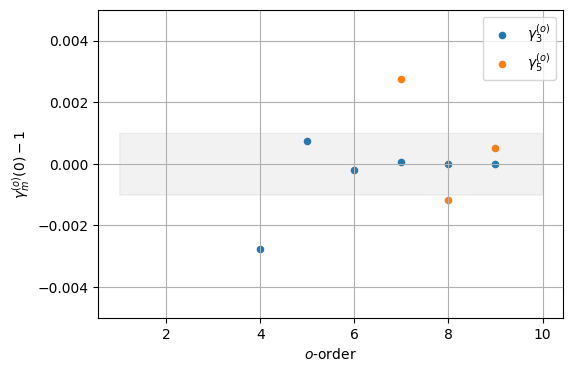
\includegraphics[width=0.6\textwidth]{fig12.png}
\caption{Evolution de $\gamma_m^{(o)}(0)$ en fonction de l'ordre $o$.}
\label{fig-gammaappat0}
\end{figure}


\begin{figure}
\centering
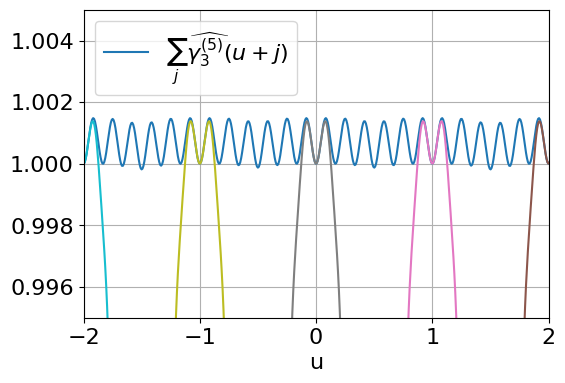
\includegraphics[width=0.6\textwidth]{fig14c.png}
\caption{Partition de l'unité pour l'approximation $\widehat{\gamma^{(5)}_3}$.}
\label{fig-gamma3-approx-unite-fourier}
\end{figure}


Cependant, si $\gamma_m(0)=1$ (ex. Eq.~\ref{eq:gamma30}), la figure \ref{fig-gammaappat0} montre que pour atteindre la précision de $\pm 0.001$ il nous faut utiliser une approximation d'ordre $o$ égale à 5 et 8 (environ) pour respectivement $m=3$ et $m=5$. Or, passer de $o$ et $o+1$ incrémente la taille du support de $\gamma_m^{(o)}(x)$ de 2 unités, car on rajoute une version de $\beta_m$ décalée aux deux extrémités du précédent support (voir le zoom de la figure \ref{fig-gamma3-approx-real}). Comme le support de $\beta_3$ (resp. $\beta_5$) est de $4$ (resp. $6$) cela signifie qu'il faudrait une approximation de $\gamma_3$ et $\gamma_5$ dont le support est multipliés d'environ un facteur $3.5$. Ce facteur est à prendre au carré dans le cas des images, soit donc un bon facteur 10 de complexité supplémentaire. Cela est bien trop prohibitif en comparaison des supports de versions cubiques et quintiques des sections précédentes. 

Ceci clôt cette section dédiée au B-Splines cardinales qui sont des outils très utilisés cependant, mais que nous omettrons dans la suite pour les raisons exposées.
%Un point qui irait dans le bon sens est que $\widehat{\gamma^{(o)}}_m(u)=(u-1)^{m+1)+O((u-1)^{m+2))$ indépendamment de l'ordre d'approximation, ce qui représenterait une meilleure évolution au voisinage de $u=1$ pour une BSpline cardinal quintique que celles obtenues avec $K_5^{bg}$ et $K_5^{je}$.
%
%Il est à noter que \cite{Costella2021} motive l'utilisation d'approximations en modifiants les coefficients $s_3(n)$ afin de procéder à des opérations sur des images codées en 8bits de Facebook et autres réseaux sociaux. Mais dans le cadre des surveys astro, les images SDSS étaient codées sur 16 bits unsigned/pixel\footnote{\url{https://classic.sdss.org/dr7/dm/flatFiles/sdR.php}} et LSST a opté pour 18 bits unsigned/pixel. Donc, il faudrait
% L'auteur a une jolie façon d'obtenir les représentations de  $\beta_m(x)$. 
%
%\begin{figure}[h]
%\centering
%\includegraphics[width=0.4\textwidth]{fig-WL1-img-non-transformed.png}
%\includegraphics[width=0.45\textwidth]{fig-WL1-pixelval-non-trans.png}
%\caption{Exemple d'une image du lot WL-1 (gauche) et la distribution afférente des valeurs de pixels (droite).}
%\label{fig-WL1-non-trans}
%\end{figure}
%\begin{figure}
%\centering
%\includegraphics[width=0.45\textwidth]{fig-WL1-pixelval-trans.png}
%\caption{Distribution des valeurs de pixels de la figure \ref{fig-WL1-non-trans} après application d'une transformation Cox-Box de paramètre $\lambda \approx -0.22$ et d'une standardisation classique.}
%\label{fig-WL1-trans}
%\end{figure}

%\begin{lstlisting}[language=iPython]
%def ANSATZ_NoCondi(L,centers,sigma,shifts,shifts_sym = False):
%    """Non conditionnal ansatz for direct estimation of energy, a scalar potential (sigmoids) + a quadratic potential
%    
%    Parameters:
%    L (int): system size = L*L 
%    centers (tensor): position of the centers of the sigmoids 
%    sigma (tensor) : width of the sigmoids
%    shifts (list of tuples) : spatial shifts for the quadratic potential, carefull (0,0) is already taken into account, do not add here  
%    shifts_sym (Bool) : if True, the shifts are not symetrized
%    """
%\end{lstlisting}
%
\subsection{Bilan: 0-\textit{padding} et ordre du noyau}
\label{sec:bilan-interpol}
%
\begin{table}
\small
\centering
\begin{tabular}{c|c|c|cc|cc|cc}
\toprule
         &         &           & \multicolumn{6}{c}{Erreur max.} \\ 
         &         &           & \multicolumn{2}{c}{"2x"} & \multicolumn{2}{|c}{"4x"} & \multicolumn{2}{|c}{"6x"} \\
noyau    & support & $u_{max}$  &   $|E_0|$ & $|\widehat{K_u}(1+u)|$ & $|E_0|$ & $|\widehat{K_u}(1+u)|$ & $|E_0|$ & $|\widehat{K_u}(1+u)|$  \\ \midrule
$K_3$    &   4     &  $2.74$   &   $0.06090$ &	 $\mathbf{0.06256}$ & $0.00449$ & 	 $\mathbf{0.00611}$ & $ 0.00092$ &  	$\mathbf{0.00160}$ \\
$K_5^{mzv}$ & 6    & $1.70$ &   $0.05446$ 	& $\mathbf{0.05638}$ & $0.00382$ & $\mathbf{0.00483}$ &  $0.00077$ 	 & $\mathbf{0.00120}$ \\
$K_5^{bg}$ & 6    & $3.62$ &   $0.02165$ 	& $\mathbf{0.03696}$ & $0.00045$ & $\mathbf{0.00123}$ &  $0.00004$ 	 & $\mathbf{0.00016}$ \\
$K_5^{je}$ & 6    & $3.69$ &   $0.02990$ 	& $\mathbf{0.01768}$ & $\mathbf{0.00064}$ & $0.00031$ &  $\mathbf{0.00006}$ 	 & $0.00003$ \\
Lanczos-3 & 6     &  $1.49$ &  $0.00012$ 	 & $\mathbf{0.01280}$ & $0.00012$ &  	$\mathbf{0.00358}$ & $0.00012$ &  	 $\mathbf{0.00353}$ \\
Lanczos-5 & 10    &  $1.08$ & $0.00360$  &  $\mathbf{0.00424}$ & $0.00005$ & $\mathbf{0.00225}$ & $0.00005$ & 	 $\mathbf{0.00122}$ \\
\bottomrule
\end{tabular}
\caption{Données chiffrées de noyaux étudiés dans la section \ref{sec:DNapprox}: outre le support, $u_{max}$ est la valeur de $|u|$ (dans l'espace de Fourier) pour laquelle les lobes ont une valeur absolue plus grande que $10^{-3}$. Les autres données indiques les valeurs maximales sur les plages $|u|<\{1/4,1/8,1/12\}$ des valeurs absolues des fonctions d'erreur (Eq.~\ref{eq:error-funct}) pour les 0-\textit{padding} de type $\times 2$, $\times 4$ et $\times 6$, respectivement. Les valeurs en gras sont les plus grandes entre les deux fonctions. Le seuil de $0.001$ est celui recherché pour choisir le noyau et le \textit{padding}.}
\label{tab-scoeff-bsplinecardapprox}
\end{table}

A ce stade, un petit rappel peut s'imposer. Il nous faut trouver une approximation du \textit{sinus cardinal} dans le cas d'une infinité d'échantillons (à la façon du théorème d'échantillonnage Sec.~\ref{sec:interpFinite}) qui agit dans l'espace de Fourier comme interpolateur. Ce noyau "imparfait" noté $K_u$ doit satisfaire deux critères élaborés dans la section \ref{sec:DNapprox}, au travers de la reconstruction d'une fonction élémentaire de type impulsionnelle $f_d(x)=a_n \delta(x-n)$ (Eq.~\ref{eq:ghosts}), à savoir pour $u=n/N\in[-1/2, 1/2]$:
\begin{align}
E_0(u) &= \sum_{j\neq 0} \widehat{K_u}(j+u)
\quad \mathrm{et}\quad  \widehat{K_u}(1+u)
\label{eq:error-funct}
\end{align}
doivent être \textitbf{tous deux en valeur absolue le plus petit possible}. Primo, pour reproduire l'image principale au mieux, et secundo faire en sorte de diminuer les images fantômes dominantes (cf. celles du premier ordre). La figure \ref{fig-E0-et-ghostsfactor} donne l'allure de ces deux fonctions d'erreur pour des noyaux étudiés. 
Juste pour montrer que les images fantômes d'ordres supérieures sont bien plus faibles, la fonction $\widehat{K_u}(2+u)$ est présentée sur la figure \ref{fig-2nd-ghostsfactor}.

On remarque immédiatement (Fig.~\ref{fig-E0-et-ghostsfactor}) que le critère d'obtenir des erreurs inférieures ou égales à $\pm 1\permil$ sur l'ensemble de la plage $[-1/2, 1/2]$ n'est pas satisfait. Mais, on peut plonger l'image initiale, pour laquelle l'échantillonnage $(a_n)$  se situe dans l'intervalle tel que $n\in\Iintv{-N/2,N/2-1}$ ($u=n/N \in [-1/2,1/2]$), dans une image plus grande constituée de zéros en dehors des $N\times N$ pixels centraux. \textbf{C'est la procédure de 0-\textit{padding}}. On augmente alors $N$ d'un facteur $2$, $4$ ou $6$ ce qui contraint respectivement les valeurs de $u$ telles que $|u|<\{1/4,1/8,1/12\}$. Ce qui est indiqué par les flèches dans les figures  \ref{fig-E0-et-ghostsfactor} et \ref{fig-2nd-ghostsfactor}. Dans ce cas, selon les noyaux, on peut trouver le facteur de \textit{padding} adéquat pour satisfaire le critère.  


Consultons alors la table \ref{tab-scoeff-bsplinecardapprox} où sont recueillies des données chiffrées permettant de comparer les différents noyaux. On se rend compte alors:
\begin{itemize}
\itemb que le noyau cubique ne peut être utilisé que s'il est associé à un \textit{padding} $\times 6$ au moins,
\itemb et que l'usage d'un \textit{padding} $\times 4$ permet d'utiliser des \textbf{noyaux "quintiques"}.
\end{itemize} 
Ces éléments constituent la principale conclusion de \cite{2014PASP..126..287B}. Cependant, le noyau préconisé était celui noté $K_5^{bg}$ (Eq.~\ref{eq:quinticBG-kernel}). Ce que l'on constate, c'est que \textbf{le noyaux $K_5^{je}$ }(Eq.~\ref{eq:quinticJE-kernel}) \textbf{obtient des scores environ deux fois meilleurs}.

\begin{figure}
\centering
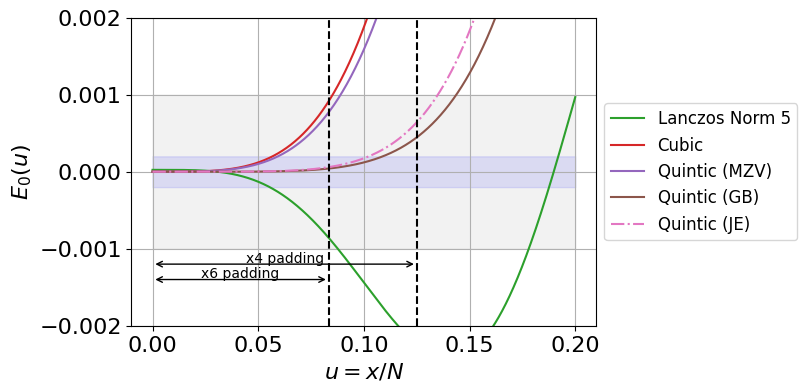
\includegraphics[width=0.9\textwidth]{fig15a.png}
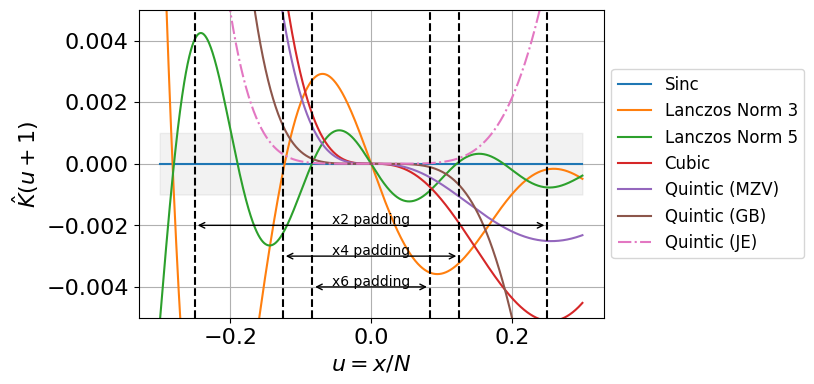
\includegraphics[width=0.9\textwidth]{fig15b.png}
\caption{Fonctions $E_0(u)$ et $\widehat{K_u}(1+u)$ pour $u=x/N\in[-1/2,1/2]$ pour des interpolants détaillés dans la section. La zone grisée indique la zone des $\pm 1\permil$.}
\label{fig-E0-et-ghostsfactor}
\end{figure}
%
\begin{figure}
\centering
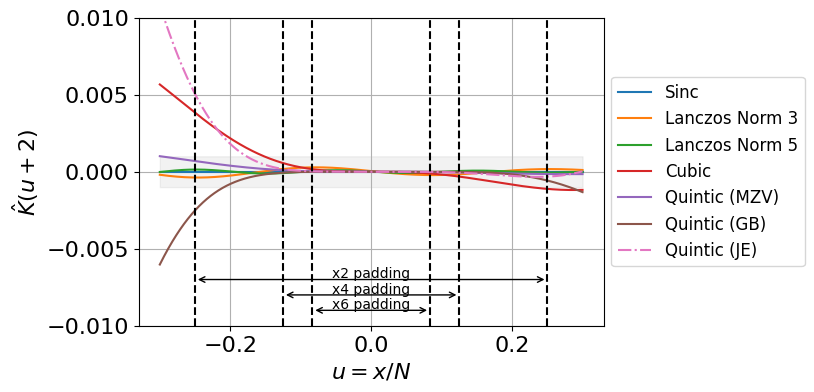
\includegraphics[width=0.9\textwidth]{fig16.png}
\caption{La fonction $\widehat{K_u}(2+u)$ dans las mêmes conditions de la figure \ref{fig-E0-et-ghostsfactor}.}
\label{fig-2nd-ghostsfactor}
\end{figure}
\begin{figure}
\centering
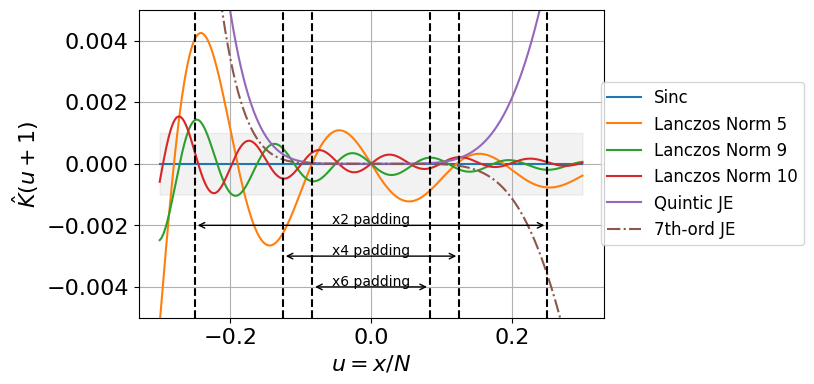
\includegraphics[width=0.9\textwidth]{fig17.png}
\caption{La fonction $\widehat{K_u}(1+u)$ dans las mêmes conditions de la figure \ref{fig-E0-et-ghostsfactor} pour quelques noyaux pour apprécier quels sont ceux pouvant utiliser un \textit{padding} $\times 2$.}
\label{fig-ghostsfactor-large-support-kernels}
\end{figure}

%
\begin{figure}
\centering
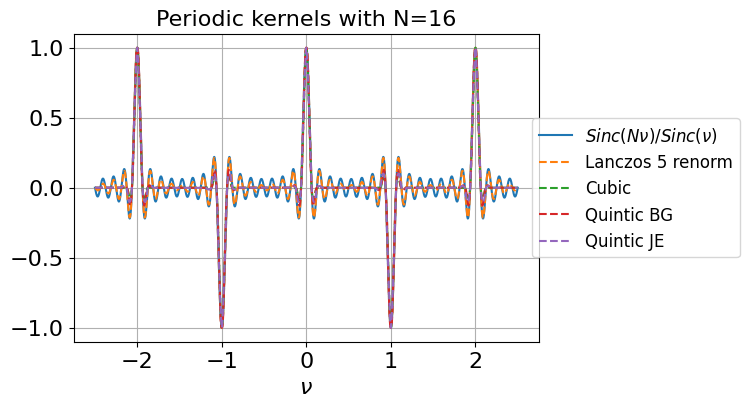
\includegraphics[width=0.8\textwidth]{fig18a.png}
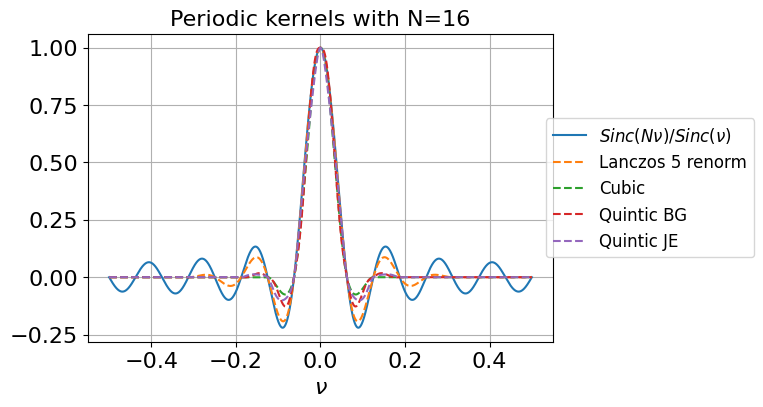
\includegraphics[width=0.8\textwidth]{fig18b.png}
\caption{Noyaux "périodisés" à la façon du sinus cardinal périodique (Eq.~\ref{eq:sinc-periodic}).}
\label{fig-periodized-kernels}
\end{figure}
%

Notons que l'article se focalise sur des noyaux de petites tailles comme on l'a motivé pour accélérer le calcul de la convolution dans l'espace de Fourier (Sec.~\ref{sec:interpFinite}). Mais, le \textit{padding} $\times 4$ peut être gourmand en mémoire, donc pour certaines applications il serait sans doute judicieux d'utiliser des noyaux de support plus grand afin de se limiter à un \textit{padding} $\times 2$. La figure \ref{fig-ghostsfactor-large-support-kernels} montre qu'il faudrait des noyaux de type Lanczos avec un paramètre $m=10$ (Sec.~\ref{sec:Lanczos}). Ce qui correspond à un noyau de support de longueur $20$ en comparaison d'un support de longueur $6$ pour des noyaux d'ordre 5. Cette augmentation de longueur de support se traduit par un facteur 10 en complexité à mettre en balance au gain d'un facteur 4 en mémoire.
%
\subsection{Cas du sinus cardinal \textit{périodique}}
\label{sec:noyaux-periodises}
%
La section précédente concernée le sinus cardinal $\sinc$ dans le cas où le nombre d'échantillons est infini. Si on se penche maintenant sur le  cas d'un nombre fini d'échantillons, nous savons que le  sinus cardinal est remplacé par sa version \textit{périodique} notée $D_N$ (Eq.~\ref{eq:sinc-periodic}). Pour remplacer $D_N$, j'utilise  la prescription suivante:
\begin{enumerate}
\item soit $K(x)$ un noyau qui dans l'espace réel est une approximation de $\sinc(x)$, alors dans un premier temps définissons
\begin{equation}
K_p(\nu) = \frac{K(N \nu)}{K(\nu)}
\end{equation}
dont le support est conditionné par celui du numérateur: si $x\in[-m,m]$ alors $\nu\in[-m/N,m/N]$.
\item Il nous faut ensuite obtenir une périodicité telle que $K_w(\nu+j) = (-1)^j\  K_p(\nu)$ pour $j\in\mathbb{Z}$ et tel que $\nu\in[-m/N,m/N]$. Remarquons que $m$ et $N$ doivent satisfaire $m/N\leq 1/2$, ce qui est en pratique le cas car $m\ll N$.    
\item Enfin, pour s'accorder sur la définition de la DFT, il faut introduire le facteur $e^{i \pi \nu}$ (voir Eq.~\ref{eq:sinc-periodic}).
\end{enumerate}
La figure \ref{fig-periodized-kernels} donne un exemple de noyaux "périodisés" avec une petite valeur $N=16$ pour illustration.
%
\section{Usage d'un noyau (in)adéquat}
\label{sec:cas-etude}
%
\subsection{Images fantômes: cas du noyaux de Lanczos}
%
Illustrons à présent l'usage des noyaux de taille limitée dans l'espace de Fourier. Prenons comme image de "galaxie", une image $N_{in}\times N_{in}$ avec $N_{in}=32$  que l'on prolonge  par \textit{0-padding} pour obtenir une image  $N_{pad}\times N_{pad}$, soit si on utilise un $\times 4$ \textit{padding} discuté dans la section précédente, $N_{pad}=128$. Le résultat est présenté dans la figure \ref{fig-128padded-init-image}.
\begin{figure}
\centering
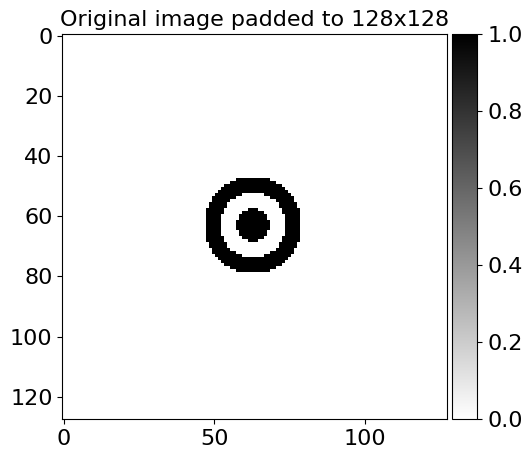
\includegraphics[width=0.6\textwidth]{fig19.png}
\caption{Image centrale $32\times 32$ complétée par \textit{0-padding} pour obtenir une image $128\times 128$.}
\label{fig-128padded-init-image}
\end{figure}

Considérons que l'on fasse à présent un échantillonnage dans l'espace de Fourier selon une grille $u_k = k \Delta u$ avec $k\in\Iintv{-M/2,M/2-1}$, telle que $\Delta u = (M \Delta x)^{-1}$, $M=512$ et $\Delta x=1$. Ce sont les paramètres pour la figure 2 de la référence \cite{2014PASP..126..287B}. On peut alors calculer $\hat{F}(u_k)$ comme résultat du produit $\hat{K}_x \times \hat{f}_d$ (rappel:  Eq.~\ref{eq:hatFu-1}) avec $K_x$ le noyau de Lanczos ($m=3$) renormalisé (Sec.~\ref{sec:Lanczos}). Pour calculer $\hat{f}_d(u_k)$ on peut alors utiliser différentes versions en lieu et place du noyau $\D_N$ (Eq.~\ref{eq:hatfdfini}).

Par exemple, la figure \ref{fig-FXlarge} compare les images de $F(x)$ dans l'espace réel, obtenues par FFT inverse de $(\hat{F}(u_k))$, où on a utilisé soit le noyau "idéal" (sinus cardinal périodique) (à gauche) soit bien le noyau périodisé à base de Lanczos d'ordre 3 (renormalisé) (à droite). Dans ce dernier cas, les images fantômes sont bien visibles. 
\begin{figure}
\centering
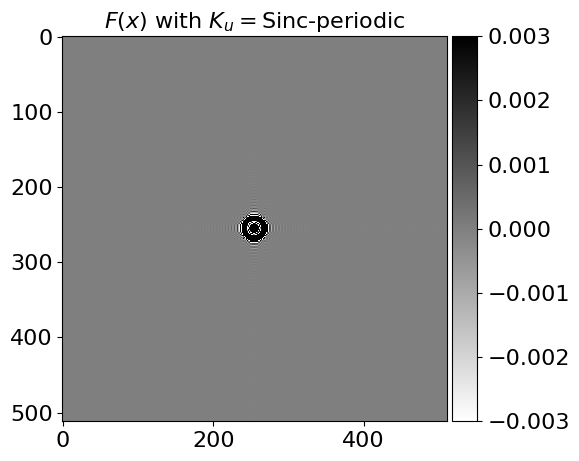
\includegraphics[width=0.45\textwidth]{fig20a.png}
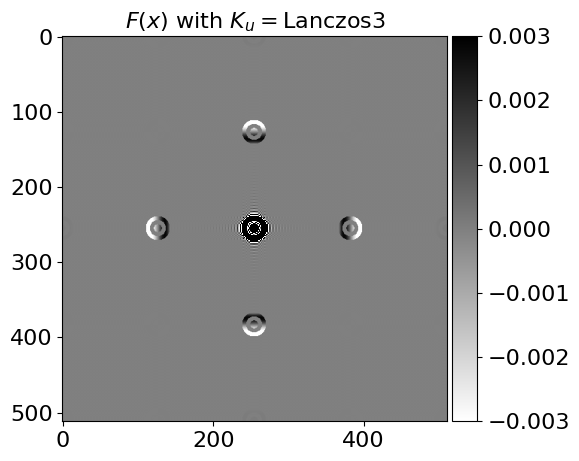
\includegraphics[width=0.45\textwidth]{fig20b.png}
\caption{Image $F(x)$ obtenue si l'on procède dans l'espace de Fourier à la convolution avec le noyau "idéal" (sinus cardinal périodique de l'équation \ref{eq:hatfdfini}), ou bien avec le noyau Lanczos-3 renormalisé  périodisés selon  la section \ref{sec:noyaux-periodises}. La LUT est restreinte à $\pm 0.003$ pour voir les images fantômes. Ici $N_{in}=32$, $N_{pad}=4\times N_{in}=128$ et $M=4\times N_{pad}=512$.}
\label{fig-FXlarge}
\end{figure}
Remarquons que dans le cas de la valeur $M=4\times N_{pad}$, les images fantômes sont situées  à une distance $N_{pad}$ de l'image centrale. Mais la position de ces images fantômes dépend de la relation entre $M$ et $N_{pad}$. Par exemple, si $M=3N_{pad}/2$, on voit les images fantômes se rapprocher de l'image centrale (Fig.~\ref{fig-FXlarge2}). Et si $M=N_{pad}/n$ avec $n$ un entier plus grand ou égal à $1$, alors \textitbf{les images s'additionnent à l'image centrale}. Ce qui dans le cas étudié ici, les images vont \textit{compenser exactement l'erreur} $E_0$ (Eq.~\ref{eq:error-funct} et Eq.~\ref{eq:ghosts}).
\begin{figure}
\centering
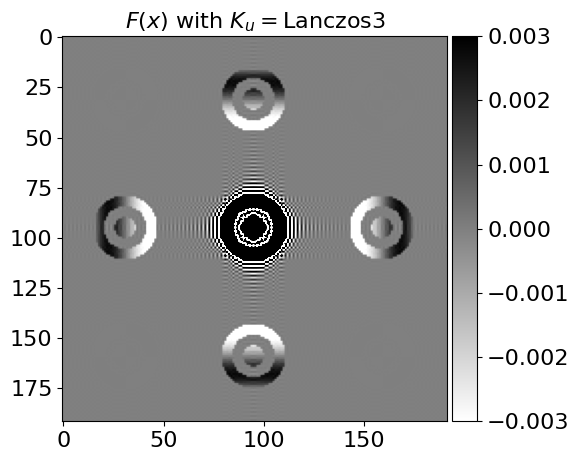
\includegraphics[width=0.45\textwidth]{fig25.png}
\caption{Conditions identiques à celle de la figure \ref{fig-FXlarge} mais ici $M=3/2 N_{pad}=192$.}
\label{fig-FXlarge2}
\end{figure}

Mais cette propriété de compensation de l'erreur sur l'image centrale par les images fantômes, n'est pas générale. En particulier, si on procède par exemple à la transformation suivante sur la grille\footnote{nb. à considérer en 2D: $(u_{1,k_1}, u_{2,k_2})$} $(u_k)_k$: 
\begin{equation}
\begin{pmatrix}
u^\prime_1 \\ u^{\prime}_2 
\end{pmatrix} = 
\begin{pmatrix}
1 & -\gamma \\ \gamma & 1
\end{pmatrix}
\begin{pmatrix}
u_1 \\ u_2 
\end{pmatrix}
\label{eq:shear}
\end{equation}
Il s'agit d'un effet de \textit{shear} dont l'origine peut être un effet gravitationnel que l'on veut mesurer précisément pour poser des contraintes sur les paramètres cosmologiques. L'effet est alors \textit{dramatique} comme on peut le voir sur la figure \ref{fig-FXlarge3}. La position des images fantômes dépendent de la valeur de $\gamma$ donc repliée sur l'image centrale produit des effets qui obèrent toute tentative de mesurer l'ellipticité de la "galaxie" soumise à la distorsion gravitationnelle.
\begin{figure}[h]
\centering
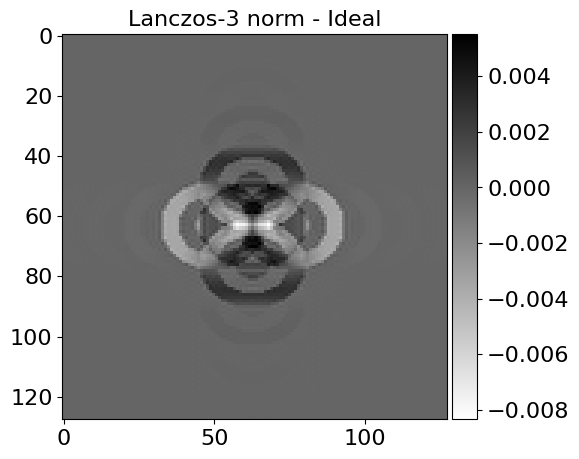
\includegraphics[width=0.45\textwidth]{fig26.png}
\caption{Conditions identiques à celle de la figure \ref{fig-FXlarge} mais ici $M= N_{pad}$ et on a appliqué la transformation linéaire de l'équation \ref{eq:shear} pouvant simulé un effet de \textit{shear} ($\gamma=0.1$ pour illustration).}
\label{fig-FXlarge3}
\end{figure}
Donc, maitriser ces images fantômes en utilisant un noyau convolutif adéquat est une tâche cruciale pour certaines applications.
%%
\subsection{Zoom sur l'image centrale et les images fantômes}
%
Pour référence, on peut procède à la différence des deux images de la figure \ref{fig-FXlarge}, pour zoomer sur l'image centrale et sur l'image fantôme de droite pour estimer l'effet des erreurs induites par l'usage d'un noyau "non-idéal". Le cas du noyau Lanczos-3 est montré sur la figure \ref{fig-FXimagette-Lanczos3}.
\begin{figure}
\centering
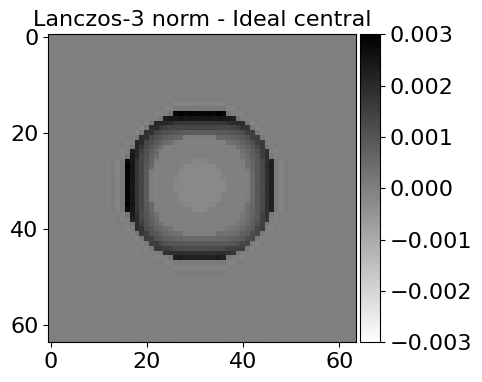
\includegraphics[width=0.45\textwidth]{fig21a.png}
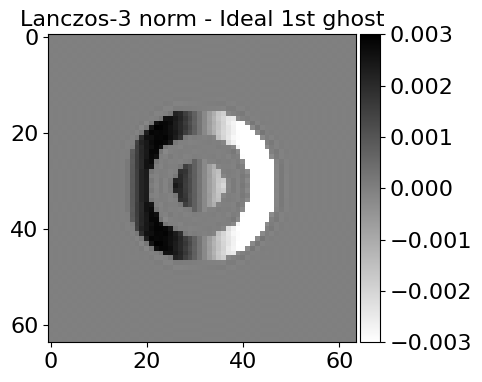
\includegraphics[width=0.45\textwidth]{fig21b.png}
\caption{Image $F(x)$ obtenu en utilisant dans le domaine de Fourier le noyau Lanczos-3 à laquelle on a soustrait l'image obtenue avec le noyau idéal, et procédé à un zoom  sur l'imagette centrale et sur une image fantôme (celle de droite de Fig.~\ref{fig-FXlarge}). La LUT est restreinte à $\pm 0.003$.}
\label{fig-FXimagette-Lanczos3}
\end{figure}

Maintenant, si l'on change le noyau de convolution, on obtient les résultats présentés sur la figure \ref{fig-FXimagette-cubique} pour le noyau cubique, sur la  figure \ref{fig-FXimagette-quinticBG} pour  le noyau de la référence \cite{2014PASP..126..287B} appelé $K_5^{bg}$ dans la section \ref{sec:BGKernels}. Ces images illustrent la motivation en fait de la référence \cite{2014PASP..126..287B} pour changer le noyau cubique par le noyau d'ordre 5 $K_5^{bg}$.
\begin{figure}
\centering
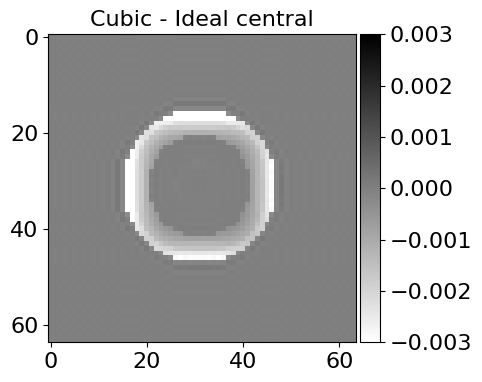
\includegraphics[width=0.45\textwidth]{fig22a.png}
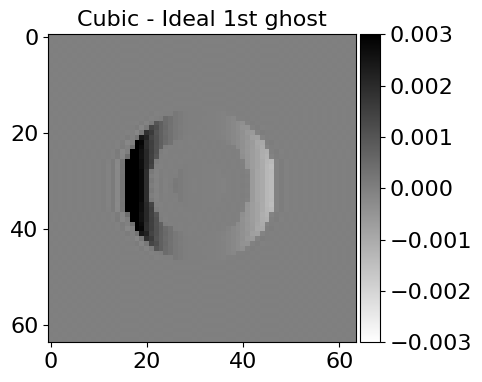
\includegraphics[width=0.45\textwidth]{fig22b.png}
\caption{Images similaires à celles de la figure \ref{fig-FXimagette-Lanczos3} en utilisant le noyau cubique en lieu et place du Lanczos-3.}
\label{fig-FXimagette-cubique}
\end{figure}
%
\begin{figure}
\centering
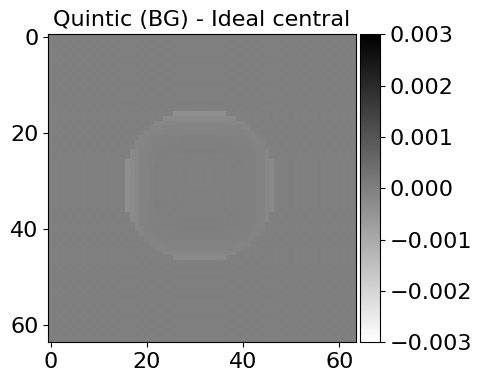
\includegraphics[width=0.45\textwidth]{fig23a.png}
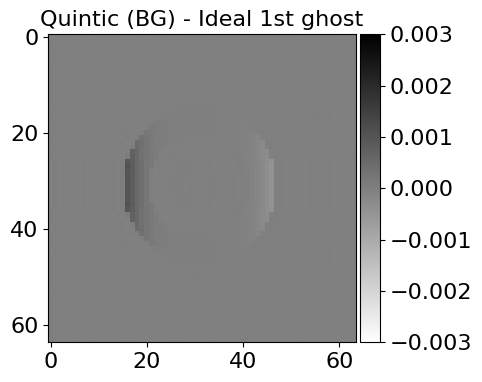
\includegraphics[width=0.45\textwidth]{fig23b.png}
\caption{Images similaires à celles de la figure \ref{fig-FXimagette-Lanczos3} en utilisant le noyau quintique  de la référence \cite{2014PASP..126..287B} de  en lieu et place du Lanczos-3.}
\label{fig-FXimagette-quinticBG}
\end{figure}

Cependant, comme indiqué dans la section \ref{sec:bilan-interpol} (Tab.~\ref{tab-scoeff-bsplinecardapprox}) le noyau $K_5^{je}$ (Sec.~\ref{sec:BGKernels}) a des performances qui \textit{a priori} sont meilleures. Pour illustrer l'impact il faut changer la LUT de $\pm 0.003$ à $\pm 0.001$. Le résultat est présenté dans la figure
\ref{fig-FXimagette-quinticJE} et montre en effet que l'impact des images fantômes est moindre en utilisant   $K_5^{je}$. 
\begin{figure}
\centering
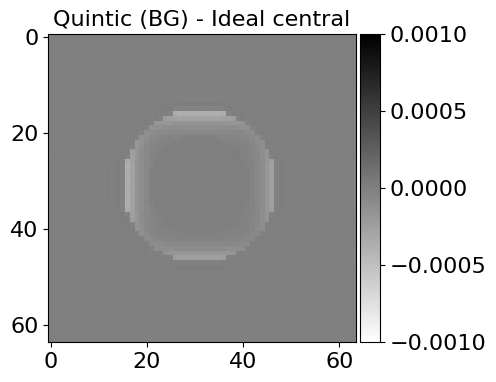
\includegraphics[width=0.45\textwidth]{fig23c.png}
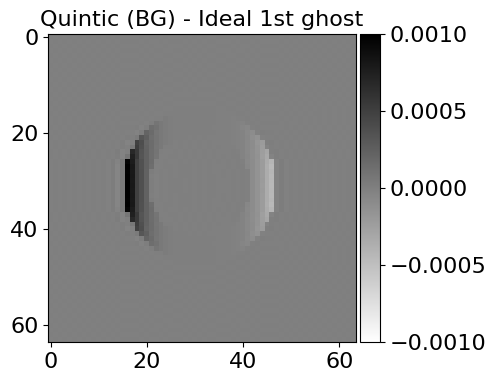
\includegraphics[width=0.45\textwidth]{fig23d.png}\\
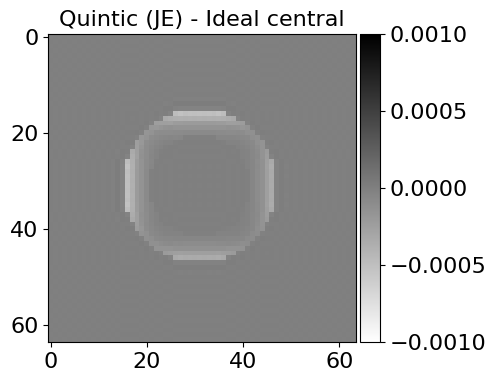
\includegraphics[width=0.45\textwidth]{fig24a.png}
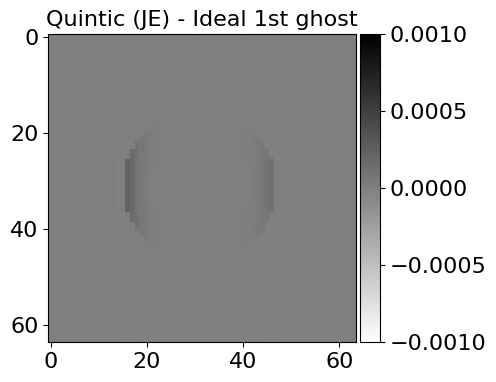
\includegraphics[width=0.45\textwidth]{fig24b.png}
\caption{Images similaires à celles de la figure \ref{fig-FXimagette-Lanczos3} en utilisant les noyaux quintiques $K_5^{bg}$ et $K_5^{je}$ en changeant la LUT en comparaison de la figure \ref{fig-FXimagette-quinticBG}.}
\label{fig-FXimagette-quinticJE}
\end{figure}
Qui plus est si l'on se place dans le cas d'un effet de \textit{shear} comme dans la figure \ref{fig-FXlarge3}, alors utiliser $K_5^{je}$ produit une réduction d'un facteur 10 de l'effet des images fantômes comme on peut le voir sur la figure \ref{fig-FXlarge-shear-QuniticJE} (attention à la LUT qui a été laissée libre dans les 2 images).
\begin{figure}
\centering
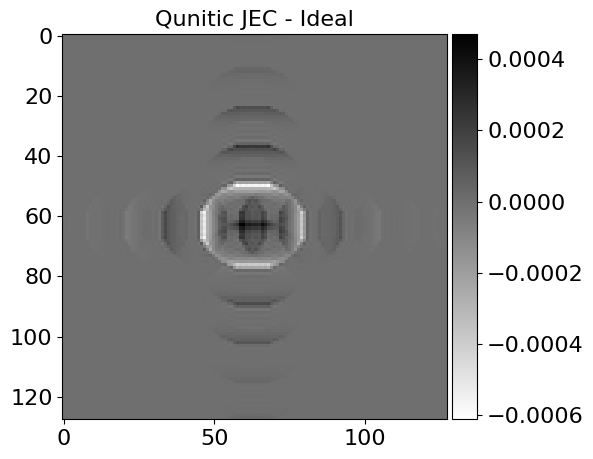
\includegraphics[width=0.45\textwidth]{fig27.png}
\caption{Conditions identiques à celle de la figure \ref{fig-FXlarge3} on changer le noyau Lanczos-3 par le noyau $K_5^{je}$. Attention à la LUT qui est différente entre les 2 images. L'effet des images fantômes est 10 fois plus faible dans le cas de $K_5^{je}$.}
\label{fig-FXlarge-shear-QuniticJE}
\end{figure}
%
\newpage
\section{Résumé}
% 
Dans cette note, j'ai repris en détails l'article de \cite{2014PASP..126..287B} concernant le choix de noyaux convolutionnels dans l'espace de Fourier. Ce type de noyau vient interpoler les coefficients de Fourier (FFT) calculés à partir d'une image 2D, soit l'échantillonnage d'une fonction sous-jacente. Cette interpolation  dans le plan de Fourier (ré-échantillonnage) est nécessaire afin d'opérer toutes sortes d'opérations, comme la convolution/déconvolution de PSF, ou bien des transformations comme celles simulant un lentillage gravitationnel. Cependant, l'opération d'interpolation nécessite d'utiliser\textit{ a priori} le noyau de Whittaker-Shannon à savoir \textit{le sinus cardinal périodique} considéré comme le noyau \textit{idéal}. Or, si on a une image initiale dans l'espace réel de taille $N\times N$, et que l'on veut une image finale de taille $M\times M$, alors la complexité est de l'ordre $O(M^2N^2)$. Ce qui motive l'emploi des noyaux alternatifs aux supports bien plus petits $n\ll N$, car alors la complexité est de l'ordre de $O(n^2 M^2)$. Cependant, ces approximations du \textit{sinus cardinal} engendrent inévitablement des artéfacts: un facteur affectant l'image de sortie, par rapport au cas idéal, et l'apparition d'images fantômes. Les intensités de ces "erreurs" sont gouvernées par les propriétés de la transformée de Fourier des noyaux alternatifs. Une bonne partie de cette note est consacrée à la recherche des noyaux pouvant satisfaire le critère double suivant: petit support, et impact minimal sur l'image de sortie. Dans ce cadre, on a pu retrouver le résultat principal de l'article de  \cite{2014PASP..126..287B} à savoir (voir Sec.~\ref{sec:bilan-interpol}): l'usage d'un noyau sous forme d'une fonction polynomiale par morceaux d'ordre 5, et d'un padding de l'image $\times 4$. Le résultat nouveau est que le choix du noyau de l'article peut être revisité et la nouvelle forme est donnée par l'expression \ref{eq:quinticJE-kernel}. Les caractéristiques comparées des noyaux sont illustrés à la fois par les données chiffrées de la table \ref{tab-scoeff-bsplinecardapprox}, et la série d'images de la section  \ref{sec:cas-etude}. Le nouveau noyau donne qualitativement et quantitativement de bien meilleurs résultats dans l'atténuation des images fantômes qui concernant le Weak Lensing sont particulièrement gênantes pour estimer la morphologie des galaxies. Ce nouveau noyau va être testé dans le cadre du software de simulation \textsf{GalSim}.

%%%%%%%%%%
\addcontentsline{toc}{section}{Références}
% Put your bibiliography file here
%\section{Bibliography}
\bibliographystyle{elsarticle-harv} %aa
\bibliography{refs.bib}

\newpage
\appendix
\section{Fourier vadémécum}
La table \ref{tag-2020-TFconv} résume quelques propriétés de la Transformée de Fourier $\mathcal{F}$ et son inverse $\mathcal{F}^{-1}$ en dimension 1. Pour simplifier les notations, il est utilisé pour désigner la TF d'une fonction $f$, $\mathcal{F}[f] = \hat{f}$. Si la Transformée inverse a la propriété $\mathcal{F}^{-1}[\mathcal{F}[f]]= \mathcal{F}[\mathcal{F}^{-1}[f]]=f$, par contre appliquer deux fois la TF a la propriété suivante: $\hat{\hat{f}}(x) = f(-x)$.

On peut également avoir besoin de:
\begin{align}
\mathcal{F}[\delta(x-x_0)](\omega) &= \reallywidehat{\delta(x-x_0)}(\omega) = N(a,b)\ e^{ibx_0\omega}\nn\\
\mathcal{F}[e^{2\pi i \nu x}](\omega) &= \reallywidehat{e^{2\pi i \nu x}}(\omega) = N(a,b)\ \delta(b/(2\pi)\omega +\nu)
\end{align}
qui dans le cas de la convention prise dans cette note $(a=0,b=-2\pi)$, donne $N(a,b)=1$ et 
\begin{align}
\reallywidehat{\delta(x-x_0)}(\omega)&=  e^{-2\pi i x_0\omega} &
\reallywidehat{e^{2\pi i \nu x}}(\omega) &=\delta(\nu - \omega) = \delta(\omega-\nu)
\end{align}



\begin{table}
\centering
{\renewcommand{\arraystretch}{2}
\begin{tabular}{cr@{\ =\ }l}
\toprule
TF & $\displaystyle\hat{f}(\omega)$ & $\displaystyle N(a,b)\int f(x) e^{i b \omega x} dx$\\
TF Inverse & $\displaystyle f(x)$ &$\displaystyle \frac{N(a,b)}{(2\pi)^a} \int \hat{f}(\omega) e^{-i b \omega x} dx$\\
TF de TF & $\widehat{\displaystyle \hat{f}(x)}(\omega)$ & $(2\pi)^a f(-\omega)$ \\
Translation & $\displaystyle\widehat{f(x-h)}(\omega)$ & $\displaystyle e^{ibw h}\hat{f}(\omega)$\\
Scaling  & $\displaystyle\widehat{f(\frac{x}{s})}(\omega)$ & $|s|\hat{f}(s\omega)$\\
Moyenne & $\displaystyle \hat{f}(0)$ & $\displaystyle N(a,b)\int f(x) \mathrm{d}x$\\
Plancherel & $\displaystyle \int f(x) g^\ast(x) \mathrm{d}x$ & $\displaystyle \frac{1}{(2\pi)^a} \int \hat{f}(\omega) \hat{g}^\ast(\omega) \mathrm{d}\omega $\\
Parseval & $\displaystyle \int |f(x)|^2 \mathrm{d}x$ & $\displaystyle \frac{1}{(2\pi)^a} \int |\hat{f}(\omega)|^2 \mathrm{d}\omega $\\
Dérivée & $\displaystyle \widehat{f^{(p)}(x)}(\omega)$ & $\displaystyle (-i b\omega)^p \hat{f}(\omega)$\\
Convolution & $\displaystyle \widehat{f\ast g}$ & $\displaystyle \frac{1}{N(a,b)} \hat{f}(\omega) \hat{g}(\omega)$\\
Multiplication par une phase & $\displaystyle \widehat{e^{i\xi x}f(x)}(\omega)$ & $\displaystyle \hat{f}(\xi/b +\omega) $\\
\bottomrule
\end{tabular}
}
\caption{Exemples des propriétés de la transformation de Fourier exprimées suivant une formulation générique tirée de Mathematica en 1D, avec la normalisation $N(a,b)=(|b|/(2\pi)^{1-a})^{1/2}$.}
\label{tag-2020-TFconv}
\end{table} 
%
\newpage
\section{Script Mathematica pour les noyaux MZV}
\label{sec:MathMZV}
Ci-dessous le code Mathematica pour générer la famille de noyaux dépendant d'un paramètre (noté "c"). Les valeurs de $m$ sont $2$, et $3$, pour les noyaux $K^{mzv}_3$ (cubique), $K^{mzv}_5$ (quintique) exposés dans la section \ref{sec:MZVkernels}.

\begin{lstlisting}[language=iPython]
FilterP[m_] := 
 Module[{a, n, condp, condn, cond, polyp, polyn, poly, h, L, vars, 
   eq1, eq2, eq3, eqs, sol},
   (* ordre du polynome *)
  n = If[m <= 1, Return["Warning: need m>1"], 2 m - 1];
  (* intervalles *)
  condp[x_] := Table[i <= x < i + 1, {i, 0, m - 1}];
  condn[x_] := Table[i < x <= i + 1, {i, -m, -1}];
  cond[x_] := Join[condn[x], condp[x]];
   (* polynomes par intervalles *)
  polyp[x_] := 
   Table[Sum[Subscript[a, j, i] x^j, {j, 0, n}], {i, 0,  m - 1}];
  polyn[x_] := 
   Table[Sum[Subscript[a, j, -i] (-x)^j, {j, 0, n}], {i, -m + 1, 0}];
  poly[x_] := Join[polyn[x], polyp[x]];
  (* le filtre par morceaux  *)
  h[x_] := 
   Evaluate@Piecewise[Table[{poly[x][[i]], cond[x][[i]]}, {i, 1, 2 m}], 0];
  (* derive *)
  h[x_, l_] := D[h[x], {x, l}];
  L = n - 2;
  (* aji variables *)
  vars =  Flatten@Table[Subscript[a, j, i], {i, 0, m - 1}, {j, 0, n}];
  (* contraintes *)
  eq1 = h[0] == 1;
  eq2 = Table[h[i] == 0, {i, 1, m - 1}];
  eq3 = Table[
    Limit[h[x, l], x -> i, Direction -> 1] == 
    Limit[h[x, l], x -> i, Direction -> -1], {l, 0, L}, {i, 0, m}];
  eqs = Flatten@{eq1, eq2, eq3, Subscript[a, n, m - 1] == c};
  (* Solve *)
  sol = FullSimplify@Solve[eqs, vars, MaxExtraConditions -> All];
  h[#] /. sol[[1]] /. #1->x
  ]
\end{lstlisting}
\section{Script Mathematica pour les noyaux BG}
\label{sec:MathBG}
Ci-dessous le code Mathematica pour générer le noyau cubique ($m=2$), la famille de noyaux quintiques  dépendant d'un paramètre ($m=3$) ainsi qu'un noyau d'ordre 7 (\textit{septic} en anglais) ($m=4$). Dans le cas de la famille de noyaux quintiques, le code fournit une solution dépendant d'un paramètre. Il est possible de faire un changement de variable en faveur de $a_{2,0}$, dans ce cas les solutions de $K_5^{bg}$ et $K_5^{je}$ exposés à la section \ref{sec:BGKernels}.

\begin{lstlisting}[language=iPython]
FilterP[m_] := 
 Module[{n, condp, condn, cond, polyp, polyn, poly, h, hat, vars, L, 
   eq1, eq2, eq3, eq3b, eq4, eq5, eq5b, eqs, sol},
   (* ordre du polynome *)
  n = If[m <= 1, Return["Warning: need m>1"], 2 m - 1];
  (* intervalles *)
  condp[x_] := Table[i <= x < i + 1, {i, 0, m - 1}];
  condn[x_] := Table[i < x <= i + 1, {i, -m, -1}];
  cond[x_] := Join[condn[x], condp[x]];
   (* polynomes par intervalles *)
  polyp[x_] := 
   Table[Sum[Subscript[a, j, i] x^j, {j, 0, n}], {i, 0, m - 1}];
  polyn[x_] := 
   Table[Sum[Subscript[a, j, -i] (-x)^j, {j, 0, n}], {i, -m + 1, 0}];
  poly[x_] := Join[polyn[x], polyp[x]];
  (* TF *)
  hat[u_] := 
   Evaluate@
    FourierCosTransform[h[x], x, u, 
     FourierParameters -> {0, -2 Pi}]; (* le filtre par morceaux  *)
  h[x_] := 
   Evaluate@
    Piecewise[Table[{poly[x][[i]], cond[x][[i]]}, {i, 1, 2 m}], 0];
  (* derivee *)
  h[x_, l_] := D[h[x], {x, l}];
  hat[u_, l_] := D[hat[u], {u, l}];
  (* aji variables *)
  vars = Flatten@Table[Subscript[a, j, i], {i, 0, m - 1}, {j, 0, n}];
  (* contraintes espace reel *)
  eq1 = {h[0] == 1};
  eq2 = Table[h[i] == 0, {i, 1, m - 1}];
  (* continuity
  in fact for x=0 the continuity leads to unconstraint for l=even, 
  and  Subscript[a, l,0]=0 for l:odd
  *)
  L = n - 4;
  eq3 = Table[
    Limit[h[x, l], x -> i, Direction -> 1] == 
     Limit[h[x, l], x -> i, Direction -> -1], {l, 0, L}, {i, 1, m}];
  eq3b = Table[Subscript[a, l, 0] == 0, {l, 1, m - 1, 2}];
  (* contraintes esapce de Fourier *)
  eq4 = {Limit[hat[u], u -> 0, Direction -> 1] == 1};
  eq5 = Table[SeriesCoefficient[hat[u], {u, 0, l}] == 0, {l, 2, n, 2}];
  eq5b = 
   Table[Evaluate@Limit[hat[u, l], u -> 1] == 0, {l, 0, n - 1}]; (* 
  Ok Gary Subscript[a, 1,2]->-1695/20 or make a20->0 *)
  (* Solve *)
  eqs = Flatten@{eq1, eq2, eq3, eq3b, eq4, eq5, eq5b};
  sol = Solve[eqs, vars, MaxExtraConditions -> All];
  {FullSimplify[sol], h[x]}
  ]
\end{lstlisting}
%%%%%%%%%%%%%%%%%%%%%%%%%%%%%%%%%

\end{document}
